% -*- Mode:TeX -*-

%% IMPORTANT: The official thesis specifications are available at:
%%            http://libraries.mit.edu/archives/thesis-specs/
%%
%%            Please verify your thesis' formatting and copyright
%%            assignment before submission.  If you notice any
%%            discrepancies between these templates and the 
%%            MIT Libraries' specs, please let us know
%%            by e-mailing thesis@mit.edu

%% The documentclass options along with the pagestyle can be used to generate
%% a technical report, a draft copy, or a regular thesis.  You may need to
%% re-specify the pagestyle after you \include  cover.tex.  For more
%% information, see the first few lines of mitthesis.cls. 

%\documentclass[12pt,vi,twoside]{mitthesis}
%%
%%  If you want your thesis copyright to you instead of MIT, use the
%%  ``vi'' option, as above.
%%
%\documentclass[12pt,twoside,leftblank]{mitthesis}
%%
%% If you want blank pages before new chapters to be labelled ``This
%% Page Intentionally Left Blank'', use the ``leftblank'' option, as
%% above. 

\documentclass[12pt,vi,twoside]{mitthesis}
\usepackage{lgrind}
%% These have been added at the request of the MIT Libraries, because
%% some PDF conversions mess up the ligatures.  -LB, 1/22/2014
\usepackage{cmap}
\usepackage[T1]{fontenc}
\usepackage{url}
\usepackage{listings}
\usepackage{multicol}
\usepackage{graphicx}
\usepackage{color}
\pagestyle{plain}

\begin{document}

% -*-latex-*-
% 
% For questions, comments, concerns or complaints:
% thesis@mit.edu
% 
%
% $Log: cover.tex,v $
% Revision 1.8  2008/05/13 15:02:15  jdreed
% Degree month is June, not May.  Added note about prevdegrees.
% Arthur Smith's title updated
%
% Revision 1.7  2001/02/08 18:53:16  boojum
% changed some \newpages to \cleardoublepages
%
% Revision 1.6  1999/10/21 14:49:31  boojum
% changed comment referring to documentstyle
%
% Revision 1.5  1999/10/21 14:39:04  boojum
% *** empty log message ***
%
% Revision 1.4  1997/04/18  17:54:10  othomas
% added page numbers on abstract and cover, and made 1 abstract
% page the default rather than 2.  (anne hunter tells me this
% is the new institute standard.)
%
% Revision 1.4  1997/04/18  17:54:10  othomas
% added page numbers on abstract and cover, and made 1 abstract
% page the default rather than 2.  (anne hunter tells me this
% is the new institute standard.)
%
% Revision 1.3  93/05/17  17:06:29  starflt
% Added acknowledgements section (suggested by tompalka)
% 
% Revision 1.2  92/04/22  13:13:13  epeisach
% Fixes for 1991 course 6 requirements
% Phrase "and to grant others the right to do so" has been added to 
% permission clause
% Second copy of abstract is not counted as separate pages so numbering works
% out
% 
% Revision 1.1  92/04/22  13:08:20  epeisach

% NOTE:
% These templates make an effort to conform to the MIT Thesis specifications,
% however the specifications can change.  We recommend that you verify the
% layout of your title page with your thesis advisor and/or the MIT 
% Libraries before printing your final copy.
\title{Performing Binary Fuzzing using Concolic Execution}

\author{Steven Valdez}
% If you wish to list your previous degrees on the cover page, use the 
% previous degrees command:
%       \prevdegrees{A.A., Harvard University (1985)}
% You can use the \\ command to list multiple previous degrees
%       \prevdegrees{B.S., University of California (1978) \\
%                    S.M., Massachusetts Institute of Technology (1981)}
\department{Department of Electrical Engineering and Computer Science}

% If the thesis is for two degrees simultaneously, list them both
% separated by \and like this:
% \degree{Doctor of Philosophy \and Master of Science}
\degree{Master of Engineering in Electical Engineering and Computer Science}

% As of the 2007-08 academic year, valid degree months are September, 
% February, or June.  The default is June.
\degreemonth{June}
\degreeyear{2015}
\thesisdate{May 18, 2015}

%% By default, the thesis will be copyrighted to MIT.  If you need to copyright
%% the thesis to yourself, just specify the `vi' documentclass option.  If for
%% some reason you want to exactly specify the copyright notice text, you can
%% use the \copyrightnoticetext command.  
%\copyrightnoticetext{\copyright IBM, 1990.  Do not open till Xmas.}

% If there is more than one supervisor, use the \supervisor command
% once for each.
\supervisor{Nickolai Zeldovich}{Associate Professor}

% This is the department committee chairman, not the thesis committee
% chairman.  You should replace this with your Department's Committee
% Chairman.
\chairman{Albert R. Meyer}{Chairman, Masters of Engineering Thesis Committee}

% Make the titlepage based on the above information.  If you need
% something special and can't use the standard form, you can specify
% the exact text of the titlepage yourself.  Put it in a titlepage
% environment and leave blank lines where you want vertical space.
% The spaces will be adjusted to fill the entire page.  The dotted
% lines for the signatures are made with the \signature command.
\maketitle

% The abstractpage environment sets up everything on the page except
% the text itself.  The title and other header material are put at the
% top of the page, and the supervisors are listed at the bottom.  A
% new page is begun both before and after.  Of course, an abstract may
% be more than one page itself.  If you need more control over the
% format of the page, you can use the abstract environment, which puts
% the word "Abstract" at the beginning and single spaces its text.

%% You can either \input (*not* \include) your abstract file, or you can put
%% the text of the abstract directly between the \begin{abstractpage} and
%% \end{abstractpage} commands.

% First copy: start a new page, and save the page number.
\cleardoublepage
% Uncomment the next line if you do NOT want a page number on your
% abstract and acknowledgments pages.
% \pagestyle{empty}
\setcounter{savepage}{\thepage}
\begin{abstractpage}
In this thesis, I designed and implemented \textit{Confuzzer}, a system that
fuzzes closed source binaries using Concolic Execution techniques in order to
find vulnerable inputs into programs that could be leveraged by attackers to
compromise systems that the binary might be running on. The system primarily
consists of a Taint and Crash Analysis tool built on top of Intel PIN, a Dynamic
Binary Instrumentation Tool, a Path Exploration system written in Python using
the z3 SMT solver to parse the tainted paths and generate symbolic equations for
those paths, and a set of nodes that receive test inputs and run the Taint/Crash
Analysis tool in order to allow for parallelization of fuzzing tasks.

\end{abstractpage}

% Additional copy: start a new page, and reset the page number.  This way,
% the second copy of the abstract is not counted as separate pages.
% Uncomment the next 6 lines if you need two copies of the abstract
% page.
% \setcounter{page}{\thesavepage}
% \begin{abstractpage}
% In this thesis, I designed and implemented \textit{Confuzzer}, a system that
fuzzes closed source binaries using Concolic Execution techniques in order to
find vulnerable inputs into programs that could be leveraged by attackers to
compromise systems that the binary might be running on. The system primarily
consists of a Taint and Crash Analysis tool built on top of Intel PIN, a Dynamic
Binary Instrumentation Tool, a Path Exploration system written in Python using
the z3 SMT solver to parse the tainted paths and generate symbolic equations for
those paths, and a set of nodes that receive test inputs and run the Taint/Crash
Analysis tool in order to allow for parallelization of fuzzing tasks.

% \end{abstractpage}

\cleardoublepage

\section*{Acknowledgments}

Thanks to Nickolai Zeldovich for supporting this work and helping find a thesis
topic and for help on the thesis project design and direction.

Thanks to Eli Davis for the initial discussions on actually implementing the
Taint analysis system using PIN. His rubber-ducking helped with the early parts
of the Confuzzer system.

This work was tested with the help of the Student Information Processing Board
for providing machines to test the distributed execution system.

%%%%%%%%%%%%%%%%%%%%%%%%%%%%%%%%%%%%%%%%%%%%%%%%%%%%%%%%%%%%%%%%%%%%%%
% -*-latex-*-

% Some departments (e.g. 5) require an additional signature page.  See
% signature.tex for more information and uncomment the following line if
% applicable.
% % -*- Mode:TeX -*-
%
% Some departments (e.g. Chemistry) require an additional cover page
% with signatures of the thesis committee.  Please check with your
% thesis advisor or other appropriate person to determine if such a 
% page is required for your thesis.  
%
% If you choose not to use the "titlepage" environment, a \newpage
% commands, and several \vspace{\fill} commands may be necessary to
% achieve the required spacing.  The \signature command is defined in
% the "mitthesis" class
%
% The following sample appears courtesy of Ben Kaduk <kaduk@mit.edu> and
% was used in his June 2012 doctoral thesis in Chemistry. 

\begin{titlepage}
\begin{large}
This doctoral thesis has been examined by a Committee of the Department
of Chemistry as follows:

\signature{Professor Jianshu Cao}{Chairman, Thesis Committee \\
   Professor of Chemistry}

\signature{Professor Troy Van Voorhis}{Thesis Supervisor \\
   Associate Professor of Chemistry}

\signature{Professor Robert W. Field}{Member, Thesis Committee \\
   Haslam and Dewey Professor of Chemistry}
\end{large}
\end{titlepage}


\pagestyle{plain}
  % -*- Mode:TeX -*-
%% This file simply contains the commands that actually generate the table of
%% contents and lists of figures and tables.  You can omit any or all of
%% these files by simply taking out the appropriate command.  For more
%% information on these files, see appendix C.3.3 of the LaTeX manual. 
\tableofcontents
\newpage
\listoffigures
\newpage
\listoftables


\chapter{Introduction}



\chapter{Existing Work}

\chapter{Design}

Foo Bar Baz

\section{Taint System Design}

Bar Baz

\section{Concolic System Design}

Baz

\chapter{Implementation}

\chapter{Evaluation}
To evaluate \textit{Confuzzer}, we compare its performance on our test cases
with the anticipated performance for blind fuzzing and other systems. We can
only calculate expected performance for blind fuzzing, since it would take
longer than available to test some of our test cases.

\begin{table}
\begin{center}
\begin{tabular}{| c | c | c | c | p{6cm} |}
\hline
Test Case & Confuzzer & Blind Fuzzing & AFL & Description\\\hline
test1 & 8 & 1.10e12 & ??? & Simple magic value test\\\hline
test2 & 6 & 1.10e12 & ??? & Keygen test using xored value\\\hline
test4 & 40494 & 1.84e19 & ??? & Toy shell example without overflow\\\hline
test4 & 40494 & 1.84e19 & ??? & Toy shell example with overflow\\\hline
\end{tabular}
\end{center}
\caption{Test Cases per Fuzzing System}
\label{table:evalcases}
\end{table}

\begin{table}
\begin{center}
\begin{tabular}{| c | c | c | c | c | p{6cm} |}
\hline
Test Case & Confuzzer & Confuzzer (Distributed) & Blind Fuzzing & AFL\\\hline
test1 & 0.21 runs/sec & 3.2 runs/sec & 2513 runs/sec & 9850 runs/sec\\\hline
test2 & 0.20 runs/sec & 3.1 runs/sec & 2497 runs/sec & 9879 runs/sec\\\hline
test3 & 0.18 runs/sec & 2.7 runs/sec & 2454 runs/sec & 10.8k runs/sec\\\hline
test4 & 0.17 runs/sec & 2.7 runs/sec & 2434 runs/sec & 11.3k runs/sec\\\hline
\end{tabular}
\end{center}
\caption{Fuzzing Speed}
\label{table:evaltime}
\end{table}

We first look at the number of test cases that our fuzzers generate, since
programs of similar complexity will have roughly the same branching amounts,
giving us a better picture of how each system scales. Our rough results are in
Figure \ref{table:evalcases}. The estimate for blind fuzzing is based on the
number of possible inputs before we are likely to hit a crashing input. We
weren't able to make measurements for AFL, since it wasn't able to determine
sufficient information to prioritize certain kinds of input, even with a basic
set of example inputs for the test application. One of the advantages of AFL is
that it is able to notify the user of crashing inputs while still running,
compared to the current implementation of Confuzzer.

We then measure the amount of time each fuzzing system takes to run test cases,
to show how the speed of the Confuzzer compares to the other systems. Figure
\ref{table:evaltime} shows that the speed of the Confuzzer system is orders of
magnitudes slower than the other systems. We actually end up having better
timing from AFL than Blind Fuzzing since it forks the binary instead of creating
a new process for every test case.

This shows how the Concolic Fuzzer system is able to hone in on specific
interesting inputs without having to hit a ton of unnecessary inputs, however
the process of finding inputs takes a long time and is heavily dependent on the
size of paths in the binary being fuzzed.

While the test cases we are using for the system are a bit artificial, there are
many existing programs that have similar constructs, including parsers that
search for magic values in order to figure out whether a file is valid, key
verification systems that check whether an input is valid to detect some key
file is valid, and even network protocols that expect a certain class of inputs.

From the timing results, we could probably end up with a more efficient system
by using a combination of \textit{Confuzzer} to generate inputs that pass
through taint checks, and then using AFL or another Fuzzer in order to look for
alternate inputs past the initial checks in the program. Unfortunately doing
this sort of merged Fuzzing requires either some amount of user input to
determine when to switch between the systems, or some sort of heuristic to deal
with moving between the fuzzers.

The results for AFL also show that its possible that moving from a PIN
instrumenter to something using QEMU User Mode Emulation might offer an
improvement in the running time of the system. Most of the slowness in running
the Confuzzer system comes from the context switching and instrumentation of the
binary code. We can increase the speed of the Fuzzer using our distributed
system to run multiple instances of the binary and Taint Analysis system. Some
of the additional improvements we can apply to \textit{Confuzzer} are covered in
the \textbf{Future Work} section in Chapter 6.

% TODO: 2/4 Pages
\chapter{Future Work}
While we currently have a working system, there is still a lot of work that can
be done to improve the overall system and create a more efficient and useful
system. Similar to the Design, we can split this into two major categories of
work, work for the Taint system and work for the Concolic Execution system.

\section{Taint Analysis Improvements}
One of the major improvements to the Taint Analysis system is to switch from
using Intel PIN to another instrumentation tool. Some options to explore, given
other Taint Analysis and fuzzing tools are using DynamoRIO as its support
improves, using full-system emulation, and finally using QEMU's user mode
emulation. The final option seems to be most likely to give improved results,
given the success that AFL has had with it.

In addition to switching the Taint Analysis to a different system, we can also
reduce the set of instructions that we have to examine by detecting standard
functions that we trust and instead of instrumenting the function execution, we
add special constraint equations to the Taint log. One example is being able to
detect strcmp and other related functions, and replacing them with constraints
that represent the possible return values from the functions, rather than having
tons of branching points and constraints within the library function
itself. There are a couple ways of doing this, from using some heuristic to
detect known functions, or actually stubbing out the real library we are
optimizing with one that has markers that the Taint Analysis tool would be able
to detect and choose to pause instrumentation.

Another improvement that needs to be made to the Taint Analysis system is
support for additional types of tainted input, either more general user input
from the console, to actual data packets through network sockets. Having these
additional forms of tainted input would allow us to test more parts of the code
without having to have artificial wrappers that convert a file input into a
network or user input.

Finally, the last major improvement to the Taint Analysis system that would be
useful is the addition of more ways to detect ``bad'' or potentially troublesome
states, some can be as simple as invalid memory access detection (which already
can be done with PIN) or even so far as detecting unintentional control flow
hijacking or policy violation. These would allow the system to detect a wider
array of potential issues all at once.

\section{Concolic Execution Improvements}
On the Concolic Execution end, one improvement is to the way we handle
constraints. If we are able to reduce the number of variables we create when
parsing the tainted assembly instructions, we could reduce some of the work z3
has to do when solving the equations. Similarly, if we are able to detect more
compound data structures, such as strings, we would be able to combine many of
the generated constraints together and use things like z3str for string
computations.

Additionally, if we were able to do better path and loop detection, we could
improve the search algorithm we use to search more interesting parts of the
program space without spending a bunch of time repeatedly working on the same
looping structure. Generally, having an improved search algorithm and
prioritization would allow us to reach interesting test cases much earlier.

Another overall improvement to the system that should be done in the future is
adapting it to work together with other existing Fuzzers. While
\textit{Confuzzer} has a advantage on some test cases that other fuzzers have
trouble with, the existing fuzzers also have their own advantages on other parts
of the program execution. Allowing multiple fuzzers to work together would allow
a wider search of the program input space without having all the test cases take
as long as the \textit{Confuzzer} test cases take.
\chapter{Conclusion}
In this thesis, we presented \textit{Confuzzer}, an implementation of a Concolic
Execution Fuzzer to help with finding inputs to the program that can cause
malicious behavior. Unlike most existing Fuzzers, Concolic Execution allows us
to get through sections of the binary that require matching certain values and
allowing us to get past sections that would otherwise cause other Fuzzers to
take a long amount of time. In implementing this system, we've aimed to design
the system to allow the analysis of as many binaries as possible, without
requiring source code to perform the analysis. While this prevents us from
constructing Intermediate Representations to use in doing the taint analysis, we
are still able to parse x86 instructions sufficiently to determine how to spread
taint through the program.

While there are still many improvements that could make to the system, the
initial prototype is already able to test a class of programs that are difficult
to test with the existing systems. Being able to programatically generate test
cases is an important step in better securing existing code and doing in-depth
testing fast enough to be effective against determined attackers.

\appendix
\chapter{Example Program}
In order to demonstrate the success of the \textit{Confuzzer} system, we've
included the code for a simple test application as well as excerpts from its
execution under the Confuzzer system. Using a single execution node, this test
took about 14 hours and generated a total of around 40500 unique inputs, without
pruning, to the program. 

\lstinputlisting[language=C++,caption=test4 Source Code]{test4.c}

This program works by taking in 8 instructions as part of a text file, each of
which could either ``[l]ist'' the files that have been created, ``[w]rite'' a
new file, or ``[d]ump'' the contents of the files. Due to an implementation bug,
this code has a memory corruption error if too many files are written. Since
this was compiled on a 64-bit system, this tends to occur when more than 4 files
are written to memory. Below is a part of the output from the fuzzer, showing
the test cases that were sent to the Taint Analyzer, as well as the newly
generated test cases from each execution:

\begin{multicols}{2}
\begin{verbatim}
Testing ./test4 with:
 Tainted input 'script.txt'
Left: 1
1 l
1 w
1 d
1 t
1 $l
1 $w
1 $d
1 $�
1 $_l
1 $_w
1 _�
1 $_d
Left: 12
2 
Left: 12
3 wl
3 ww
3 wd
3 wt
3 w$l
3 w$w
3 w$d
3 w$�
3 w$_l
3 w$_w
3 w$_d
3 w$_t
3 w$__l
3 w$__w
3 w$__d
3 w$_c�
3 w$�__l
3 w$�__w
3 w$�__d
3 w$P�C�
3 w$O_?_l
3 w$O_?_w
3 w$O_?_d
3 w$__c`�
3 w$_____l
3 w$_____w
3 w$_____d
3 w$___�?_
Left: 39
4 �
Left: 39
5 $_t
5 $__l
5 $__w
5 $__d
5 $_c�
5 $�__l
5 $�__w
5 $�__d
5 $P�C�
5 $O_?_l
5 $O_?_w
5 $O_?_d
5 $__c`�
5 $_____l
5 $_____w
5 $_____d
5 $_X_c_�
5 $___�?_l
5 $___�?_w
5 $___�?_d
5 $`______
Left: 59
...
Left: 5
Left: 4
Left: 3
Left: 2
Left: 1
40481 wwwwwwl
40481 wwwwwww
40481 wwwwwwd
40481 wwwwwwt
40481 wwwwww$l
40481 wwwwww$w
40481 wwwwww$d
40481 wwwwww$_
Left: 8
40482 wwwwwwll
40482 wwwwwwlw
40482 wwwwwwld
40482 wwwwwwl$
Left: 11
Left: 10
Left: 9
Left: 8
40486 wwwwww$l
40486 wwwwww`
Left: 9
Left: 8
40488 wwwwwwd
Left: 8
Left: 7
Left: 6
Left: 5
40492 wwwwwwl^D
Left: 5
Left: 4
40494 wwwwwwl$
Left: 4
Left: 3
Left: 2
Left: 1
\end{verbatim}
\end{multicols}

A subset of the crashing inputs that were discovered is below:

\begin{verbatim}
Crashing Inputs:
        $_wwwwdw
        $_wwwwlw
        $wdwwwdw
        $wdwwwwl
        $wldwwww
        $wlw_www
        $wlwdwww
        $wlww_ww
        $wlwwww
...
\end{verbatim}

This along with the remaining crashing inputs covers most of the space of inputs
that should crash the program, showing that even with a program that has a
combinatorial explosion of paths $4^8$, Confuzzer is still able to function in a
reasonable amount of time. The 14 hours for $~40000$ paths matches closely with
the results observed by the SAGE system \cite{sage}. With the use of N nodes,
the time needed to run this test could be reduced by about a factor of $N$,
since the majority of the time was spent in the actual execution of the programs
with different inputs.
\chapter{Example Execution Graphs}
Attached is the code and execution graphs for some of the simpler test cases
we've been using.

\lstinputlisting[language=C++,basicstyle=\tiny,caption=test1 Source Code]{test1.c}

\lstinputlisting[language=C++,basicstyle=\tiny,caption=test2 Source Code]{test2.c}

\begin{figure}[ht]
 \centering
 \begin{tabular}{| c | c |}
   \hline
   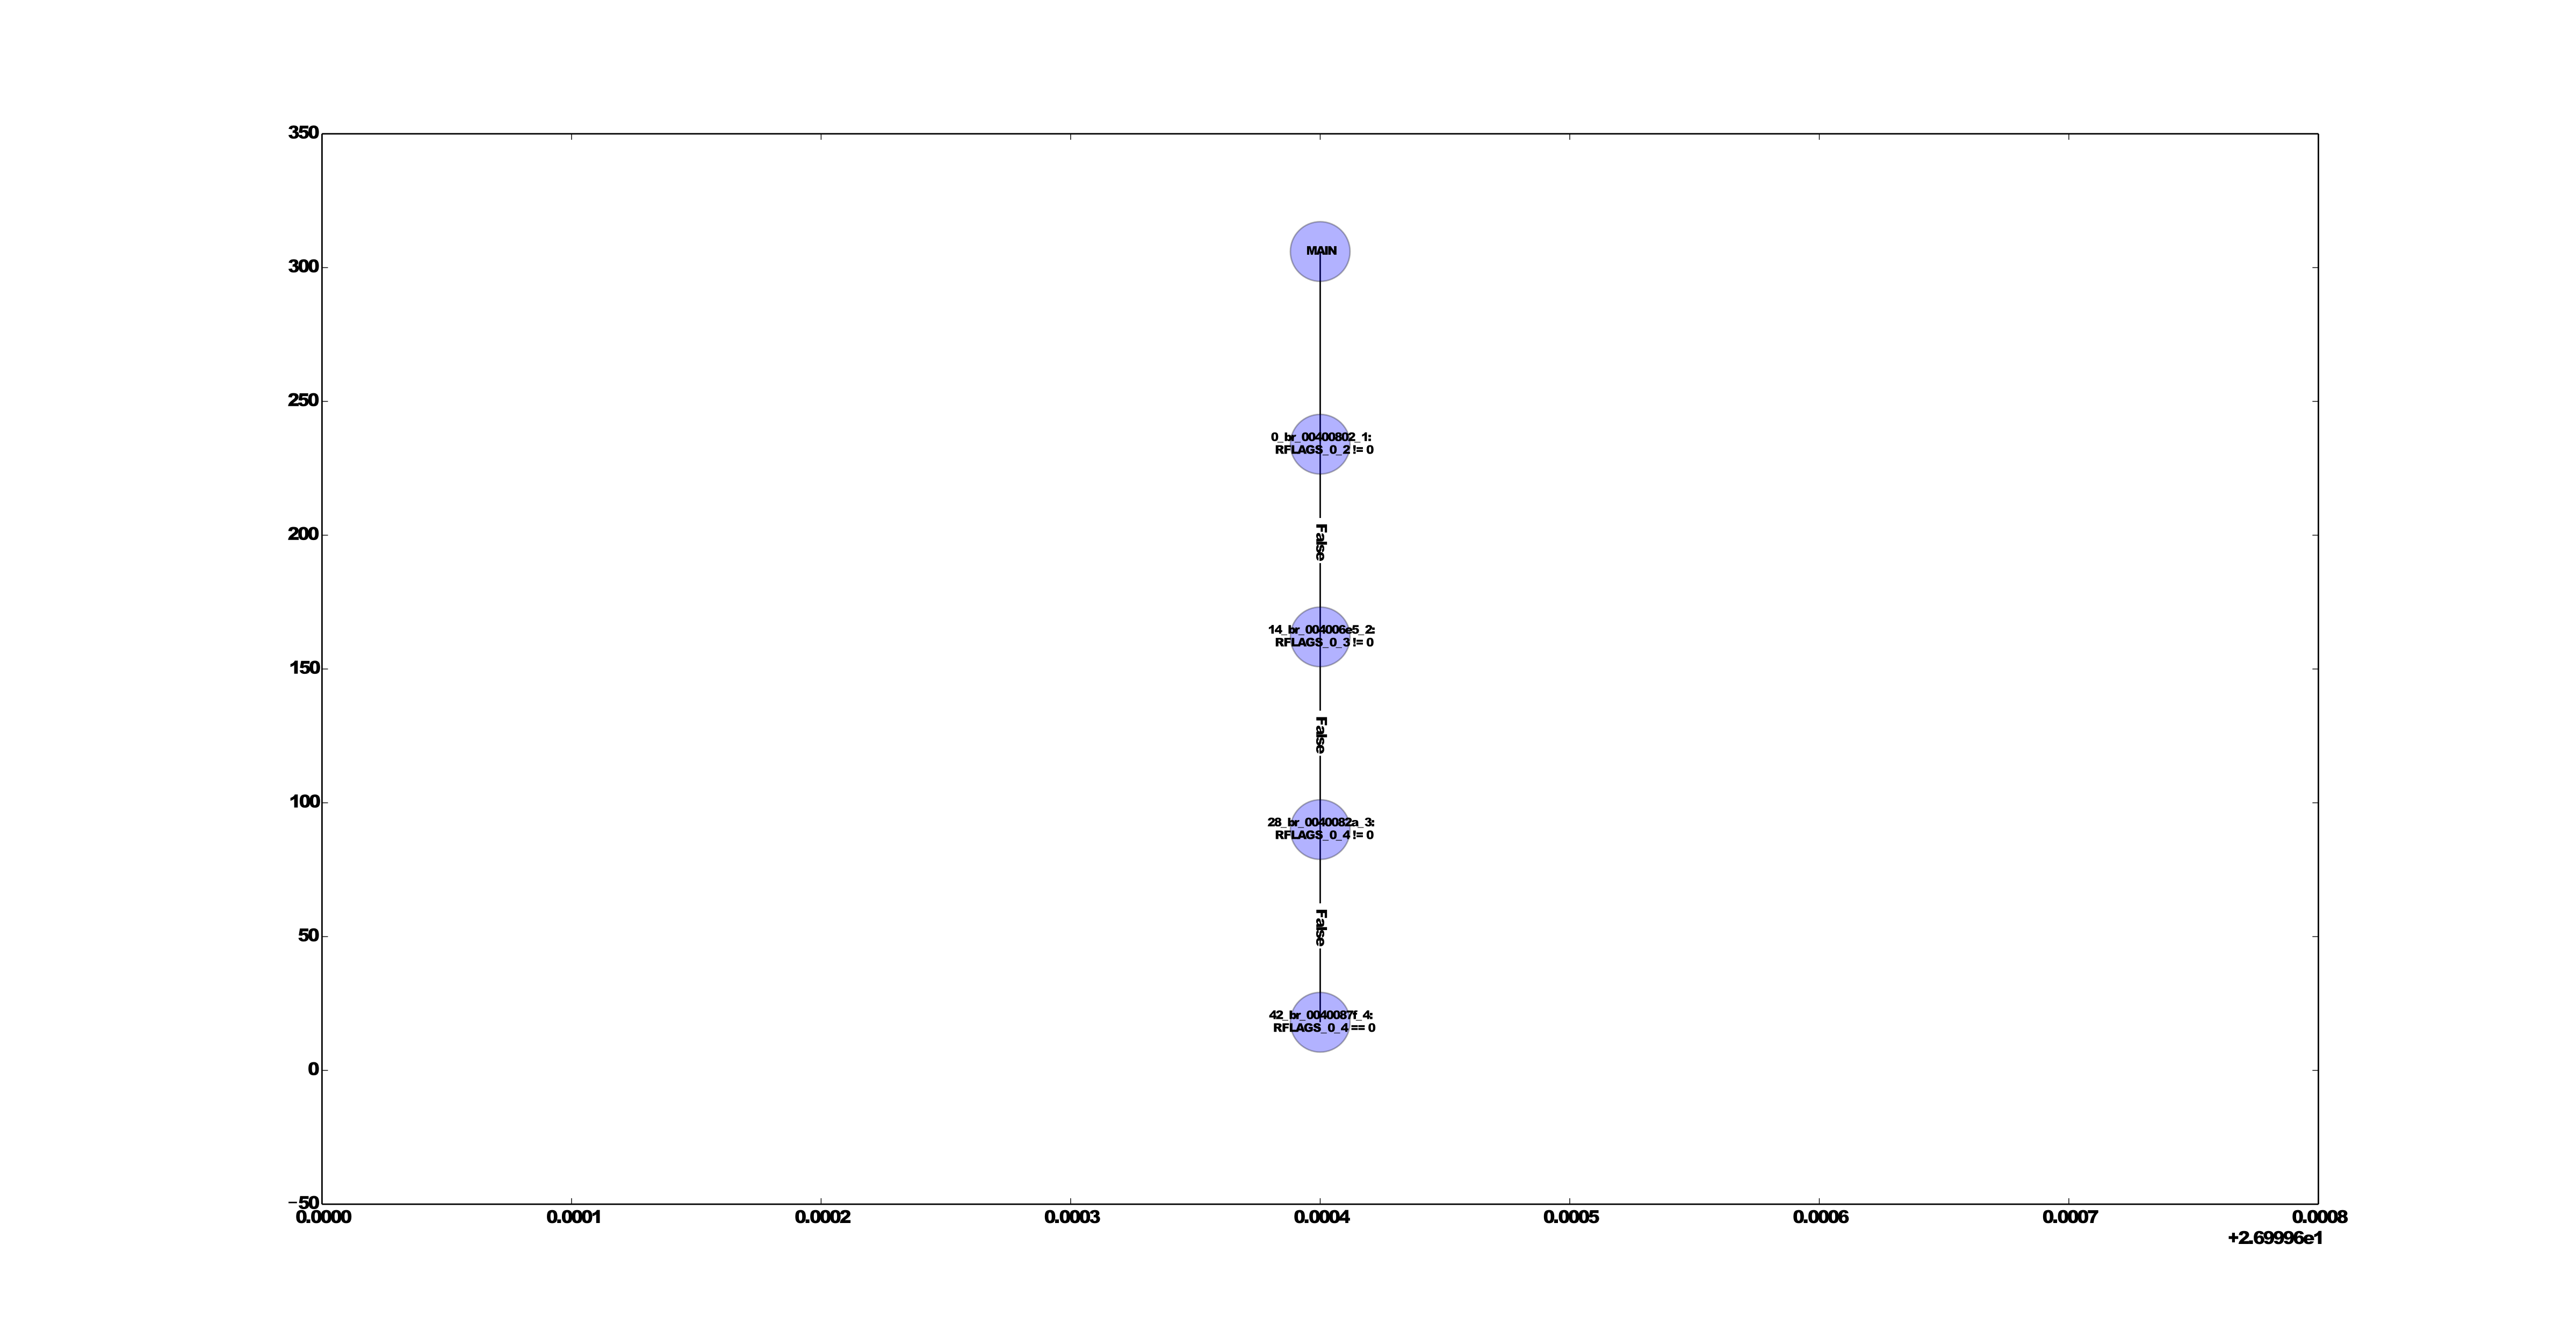
\includegraphics[width=0.45\textwidth]{graphs/1_0}
   &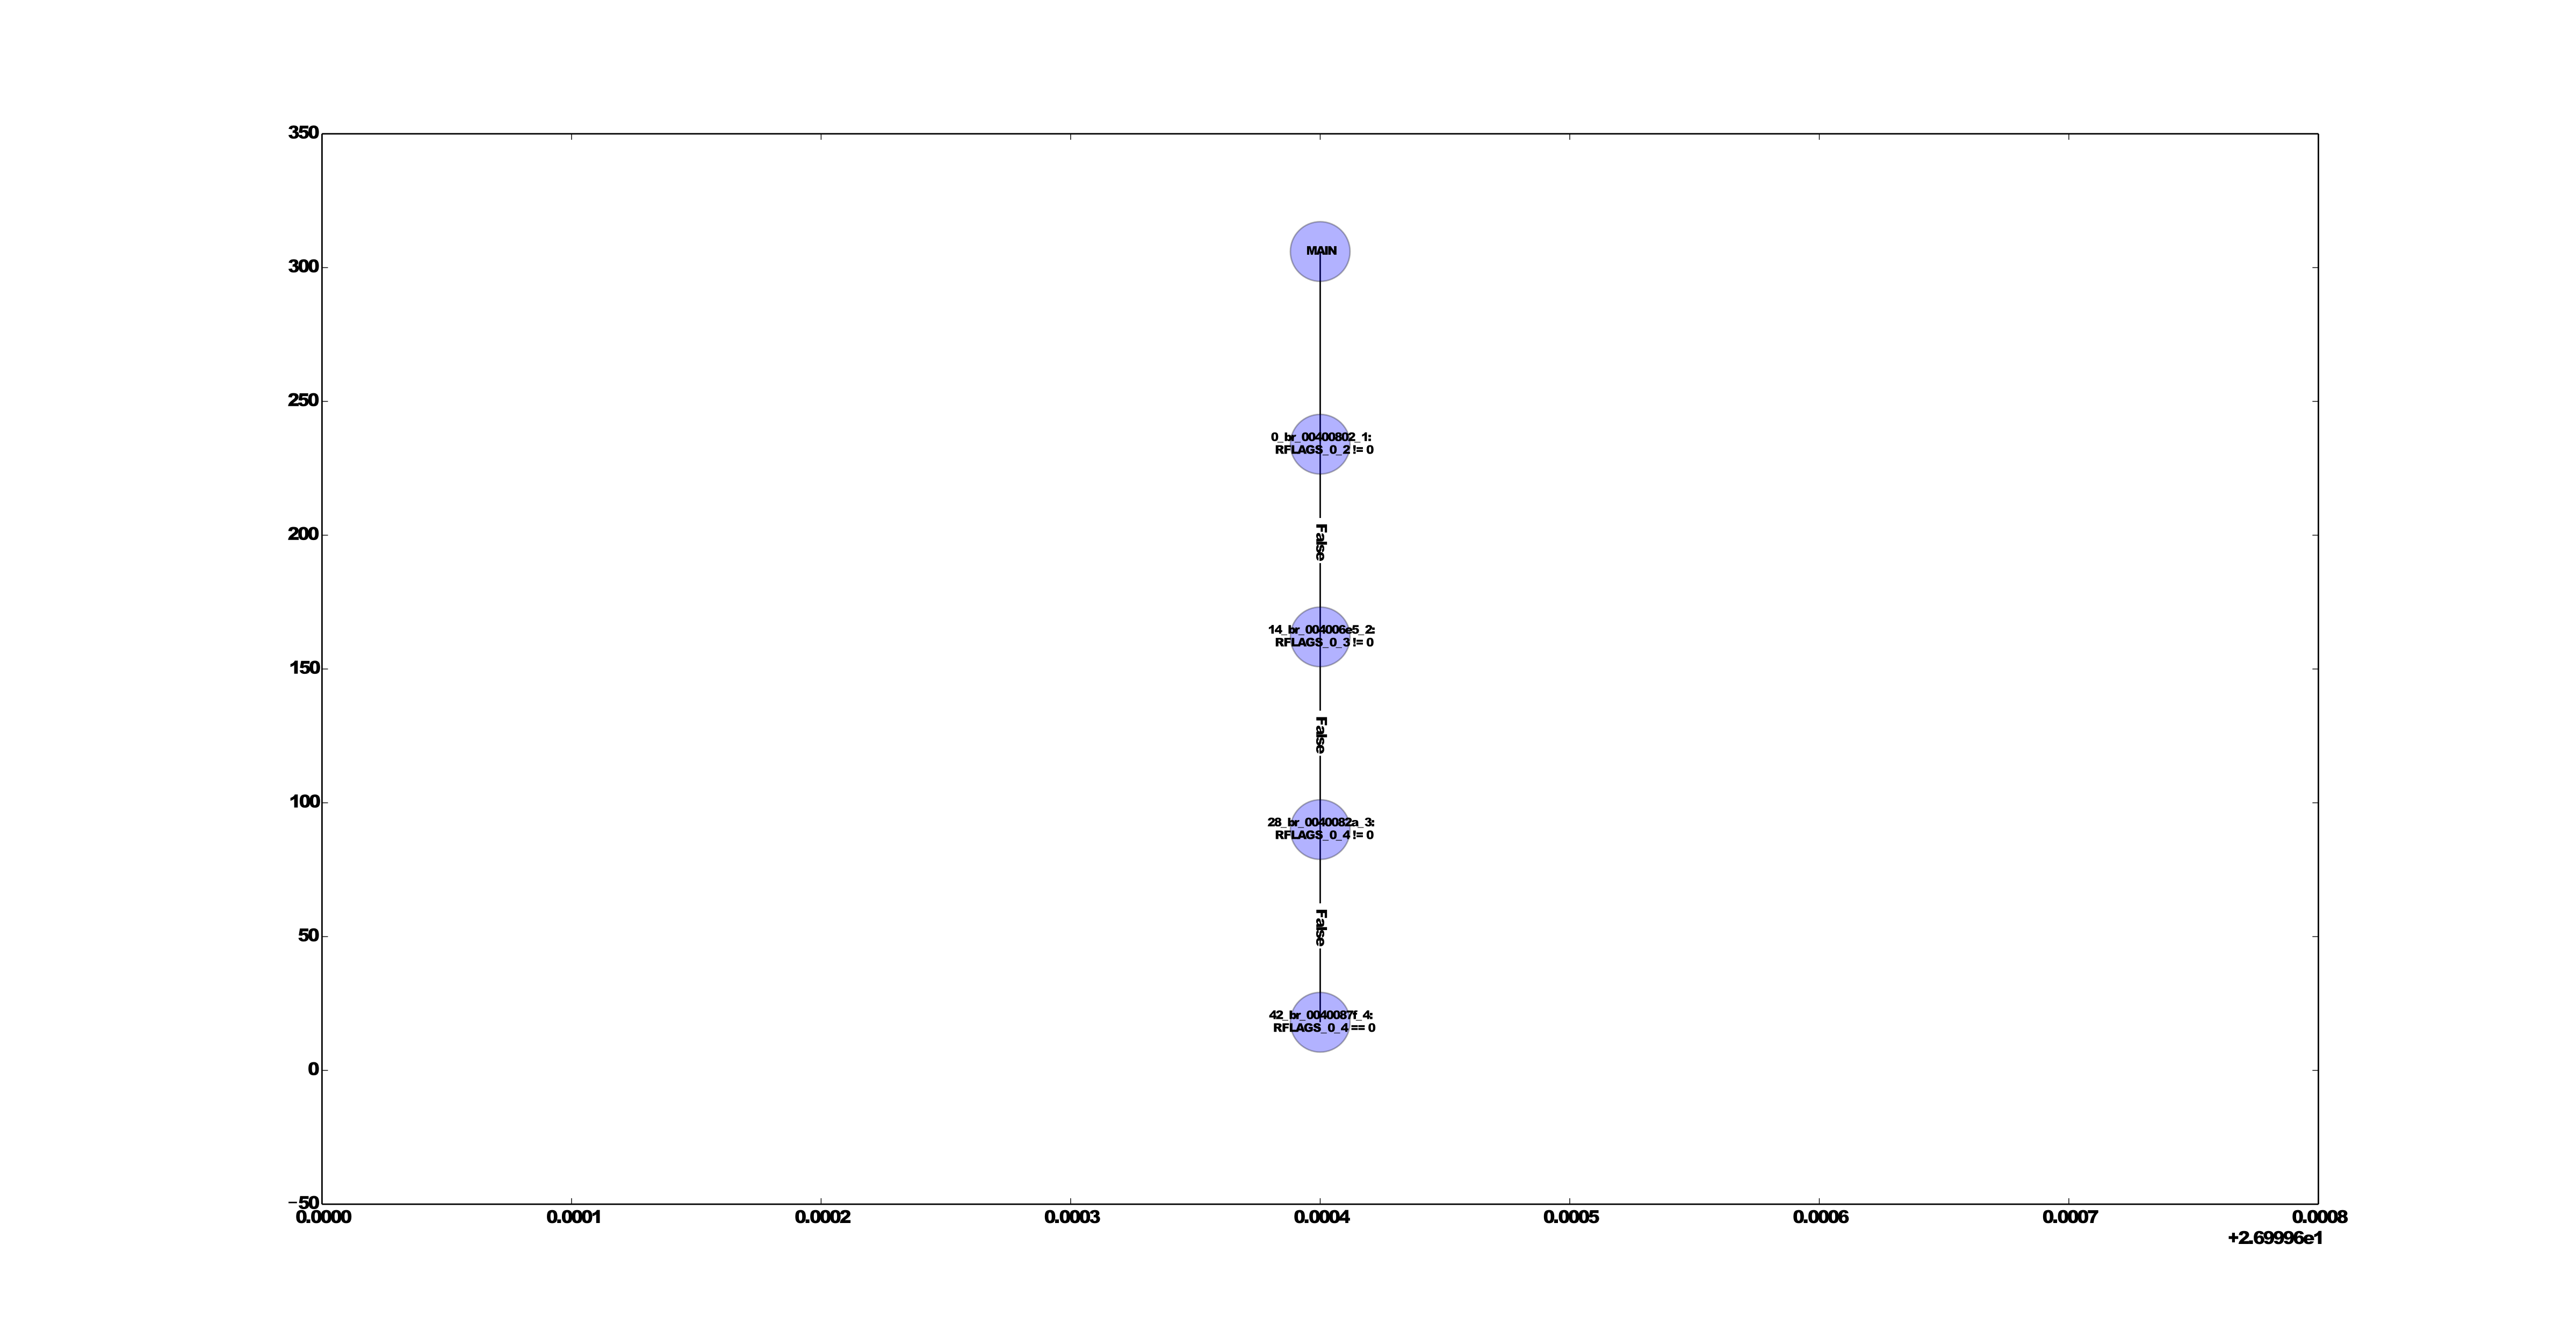
\includegraphics[width=0.45\textwidth]{graphs/1_1}\\\hline
   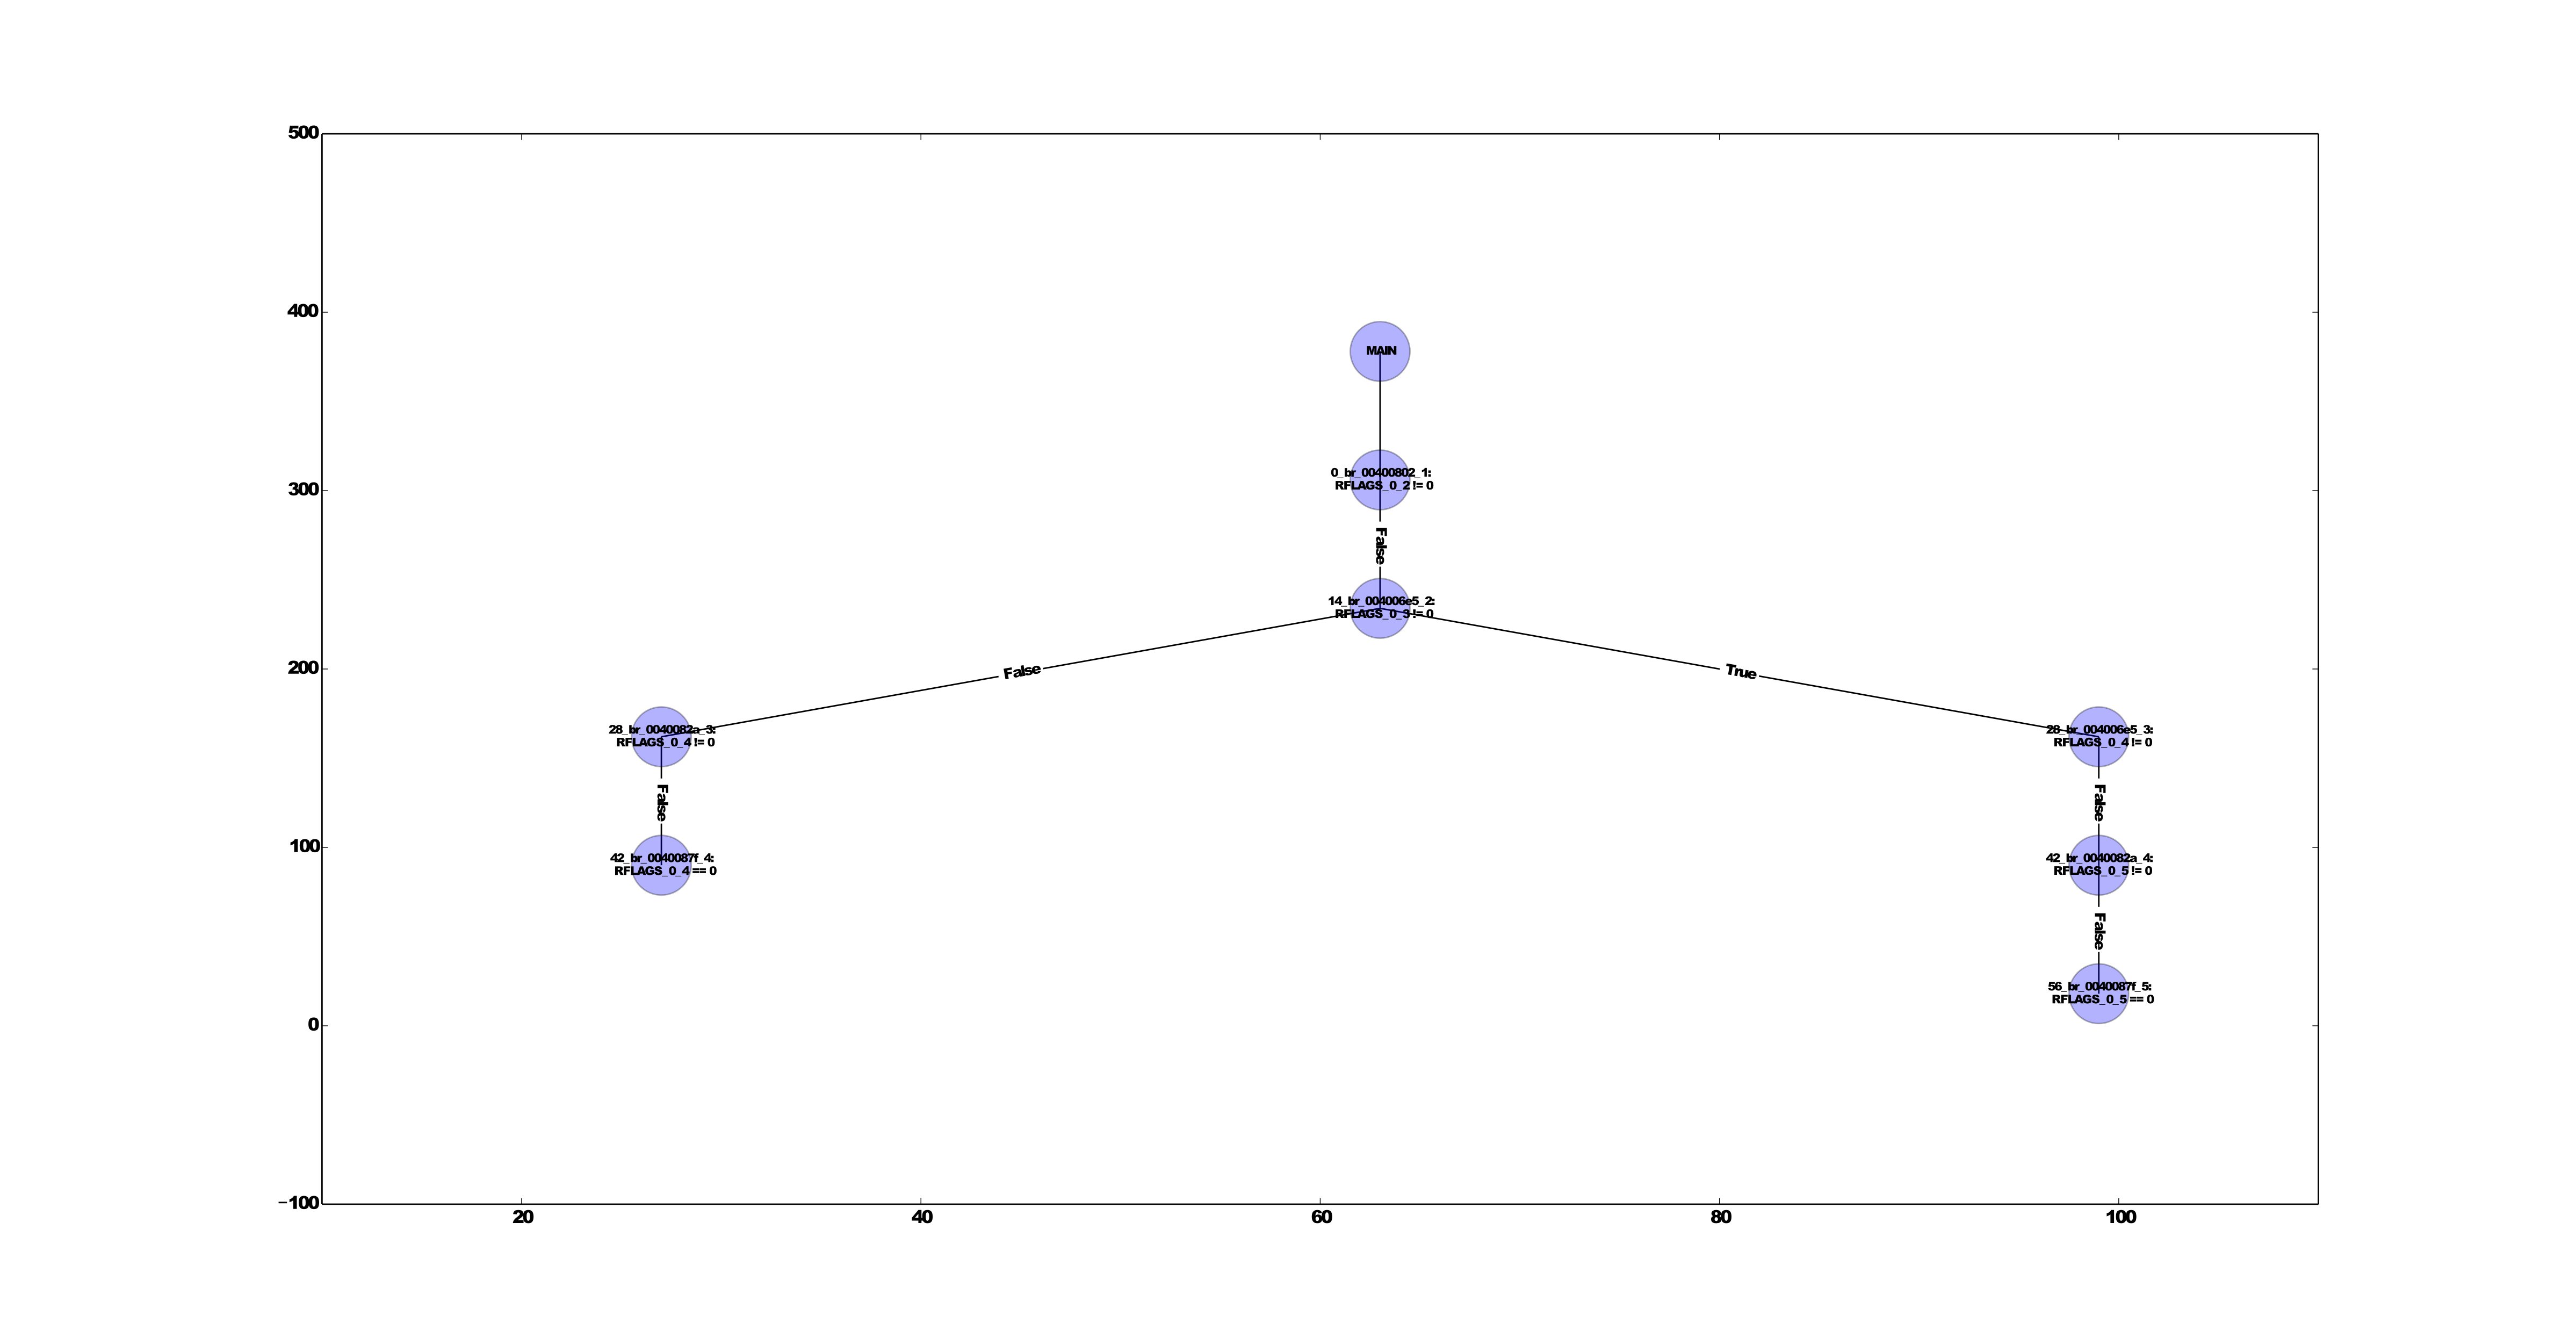
\includegraphics[width=0.45\textwidth]{graphs/1_2}
   &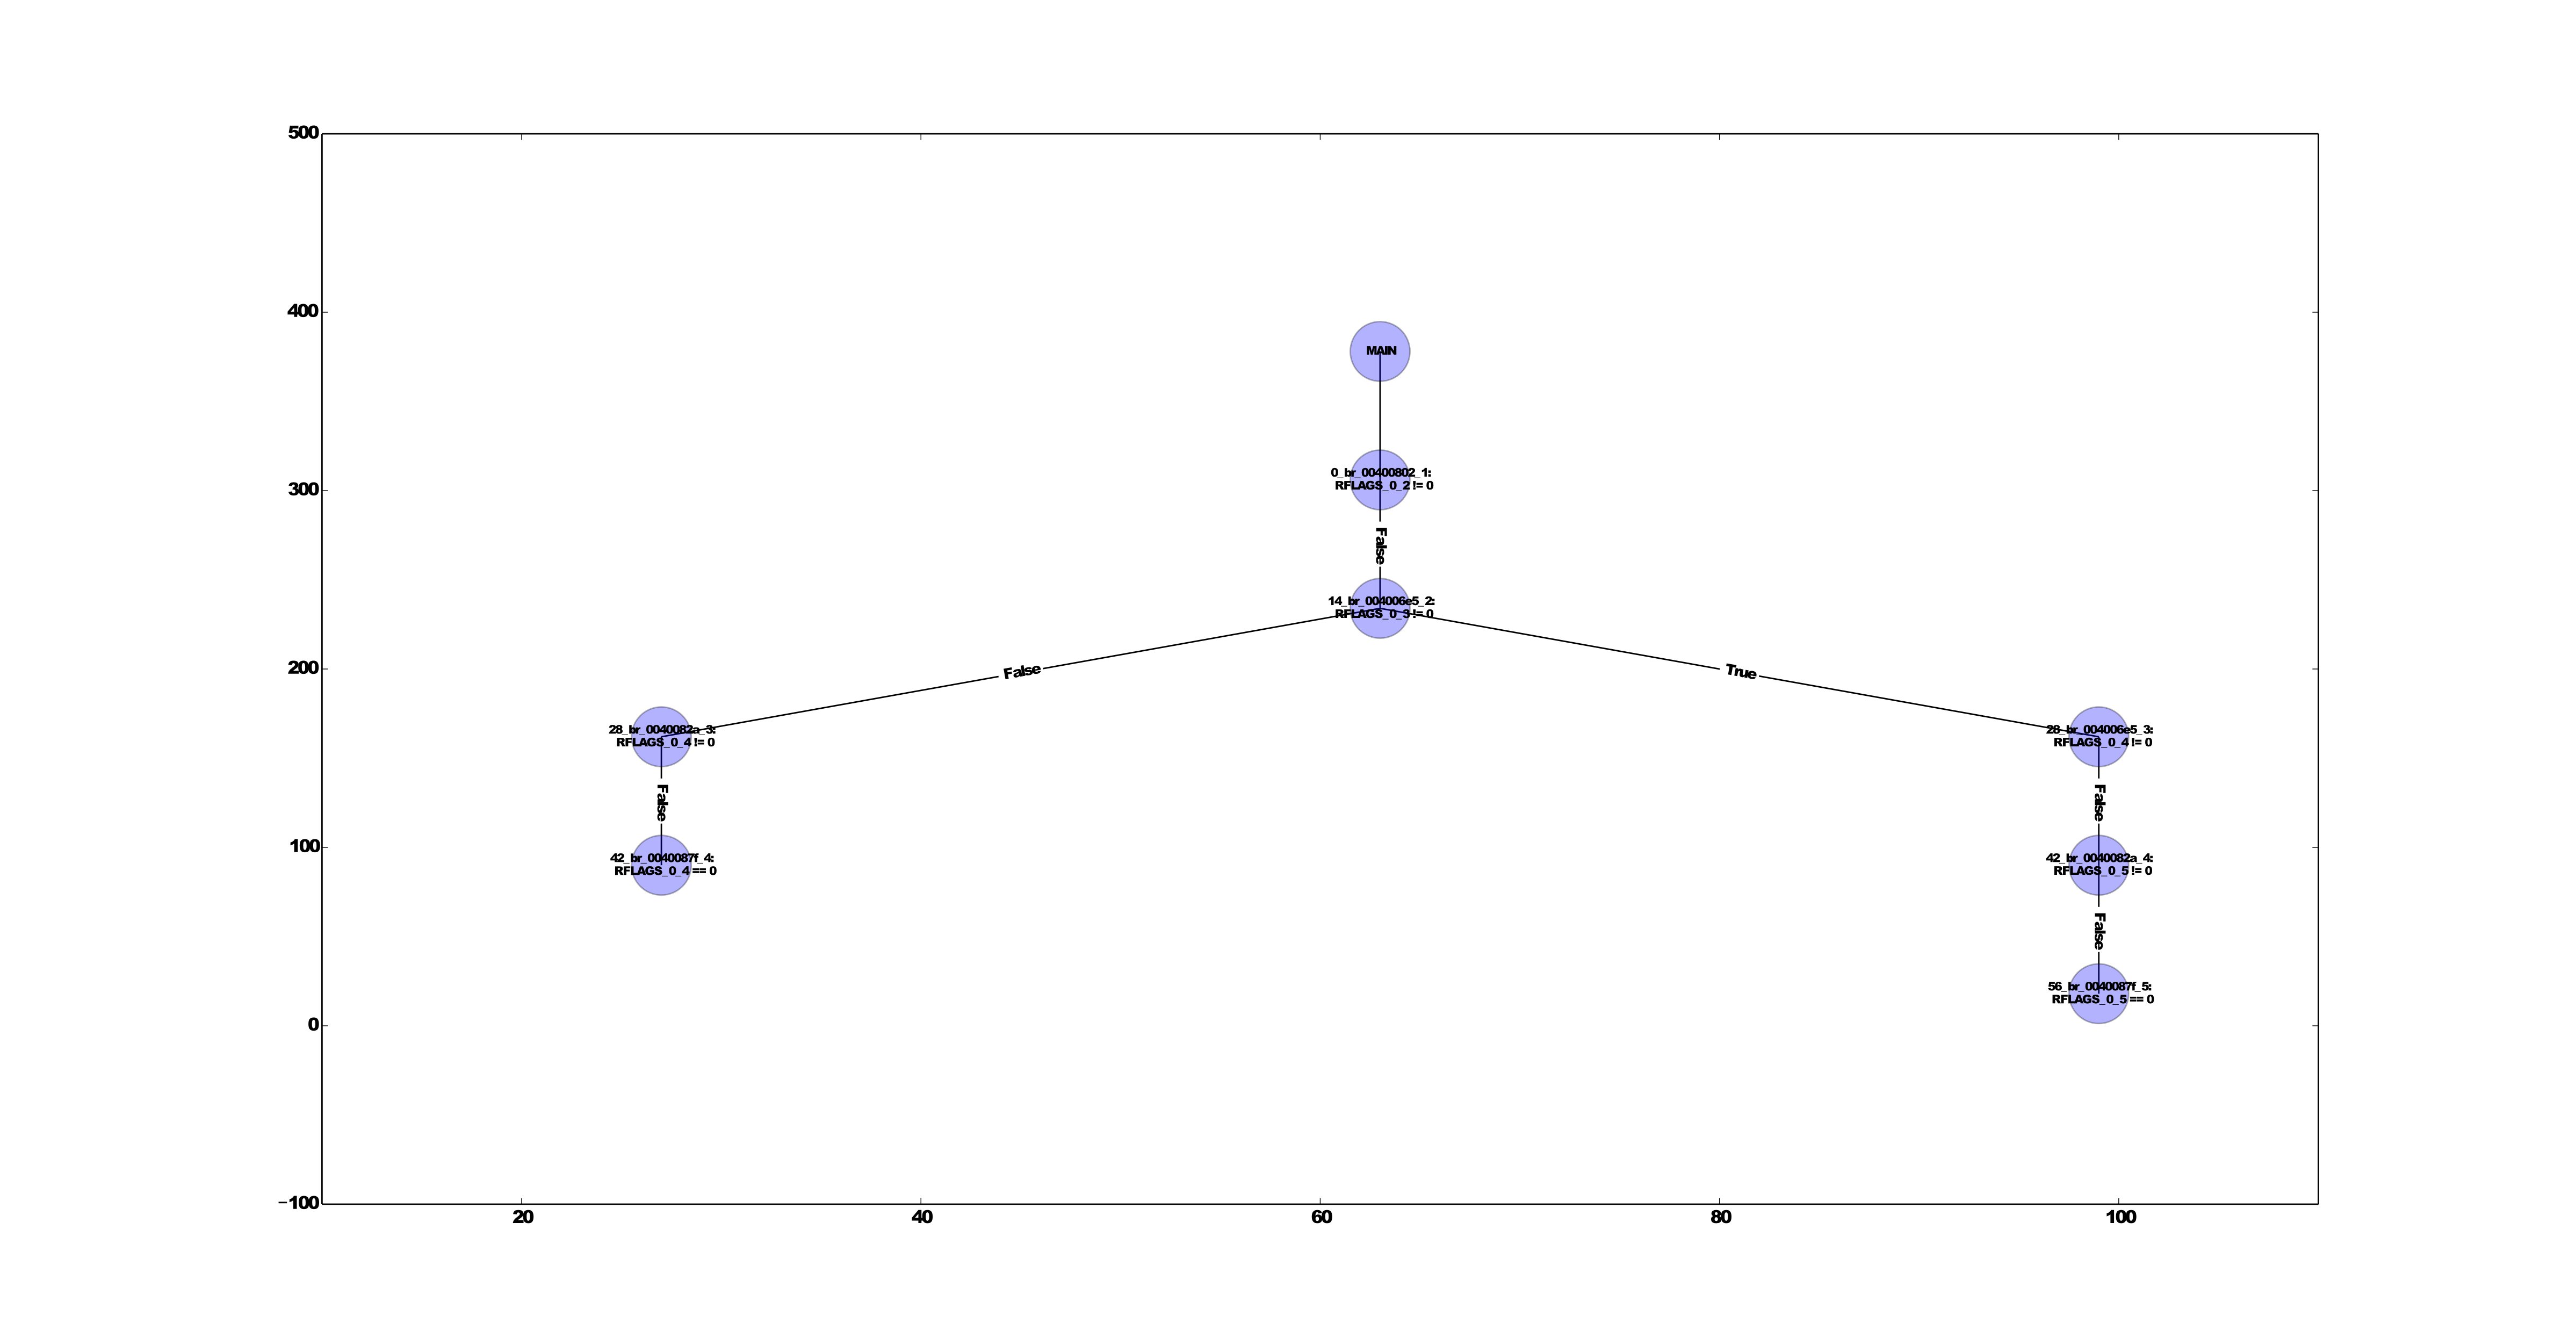
\includegraphics[width=0.45\textwidth]{graphs/1_3}\\\hline
   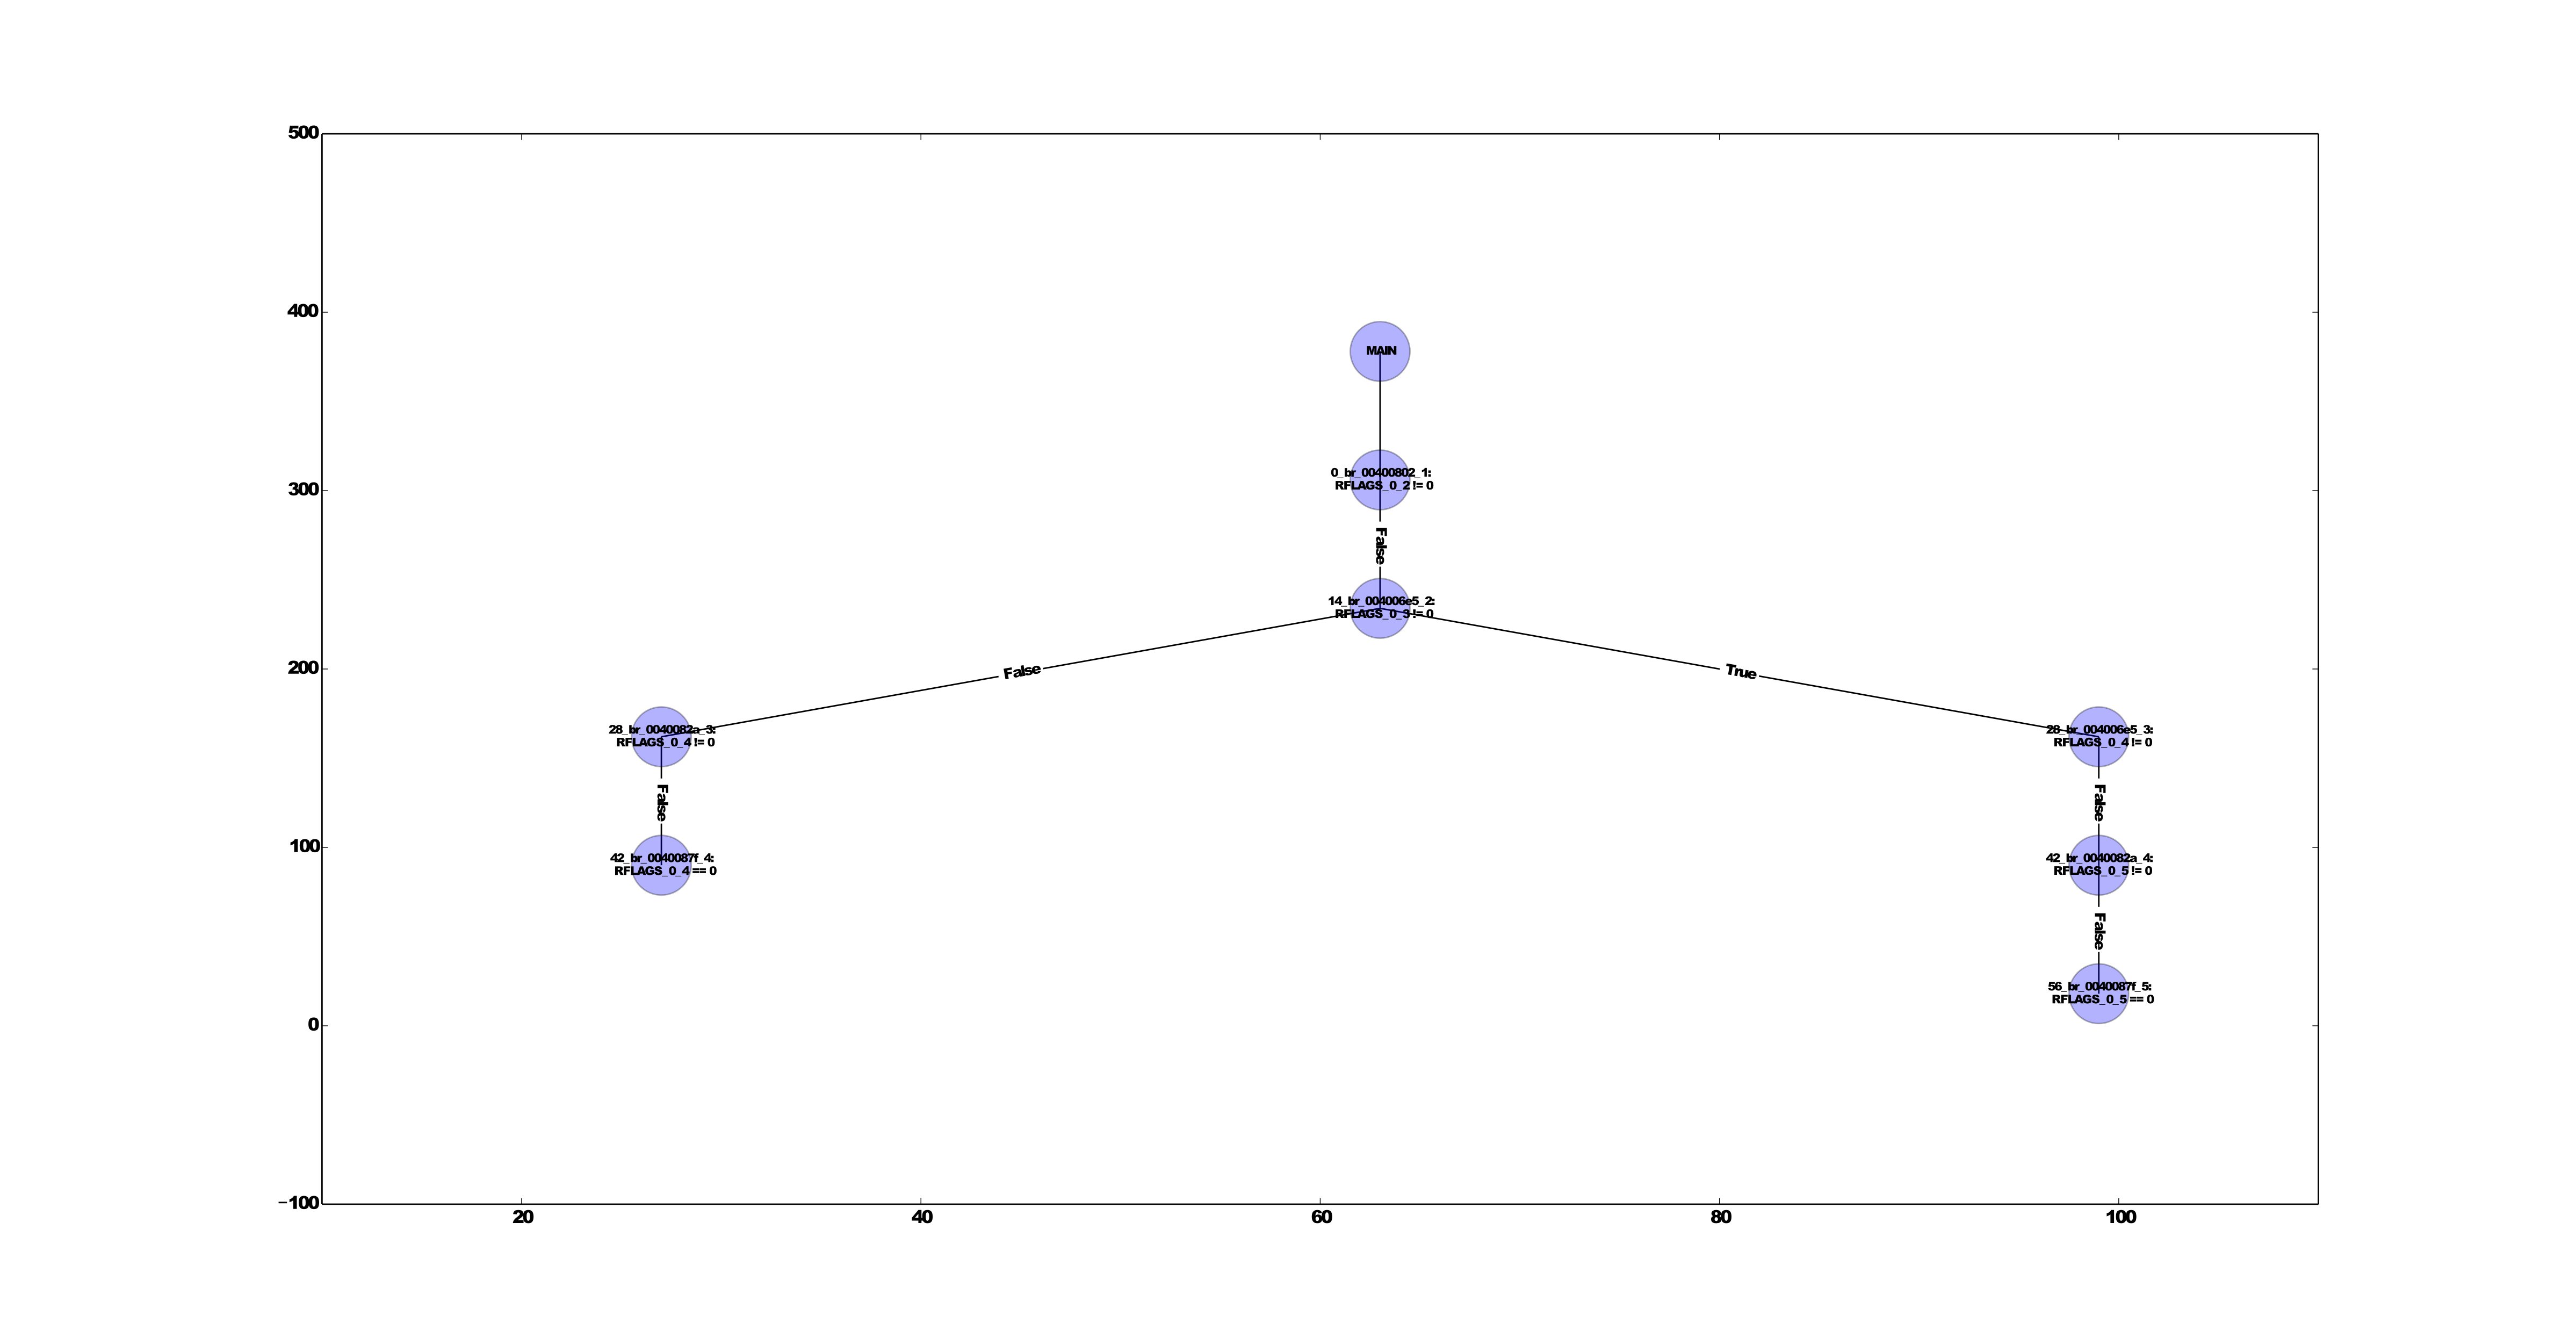
\includegraphics[width=0.45\textwidth]{graphs/1_4}
   &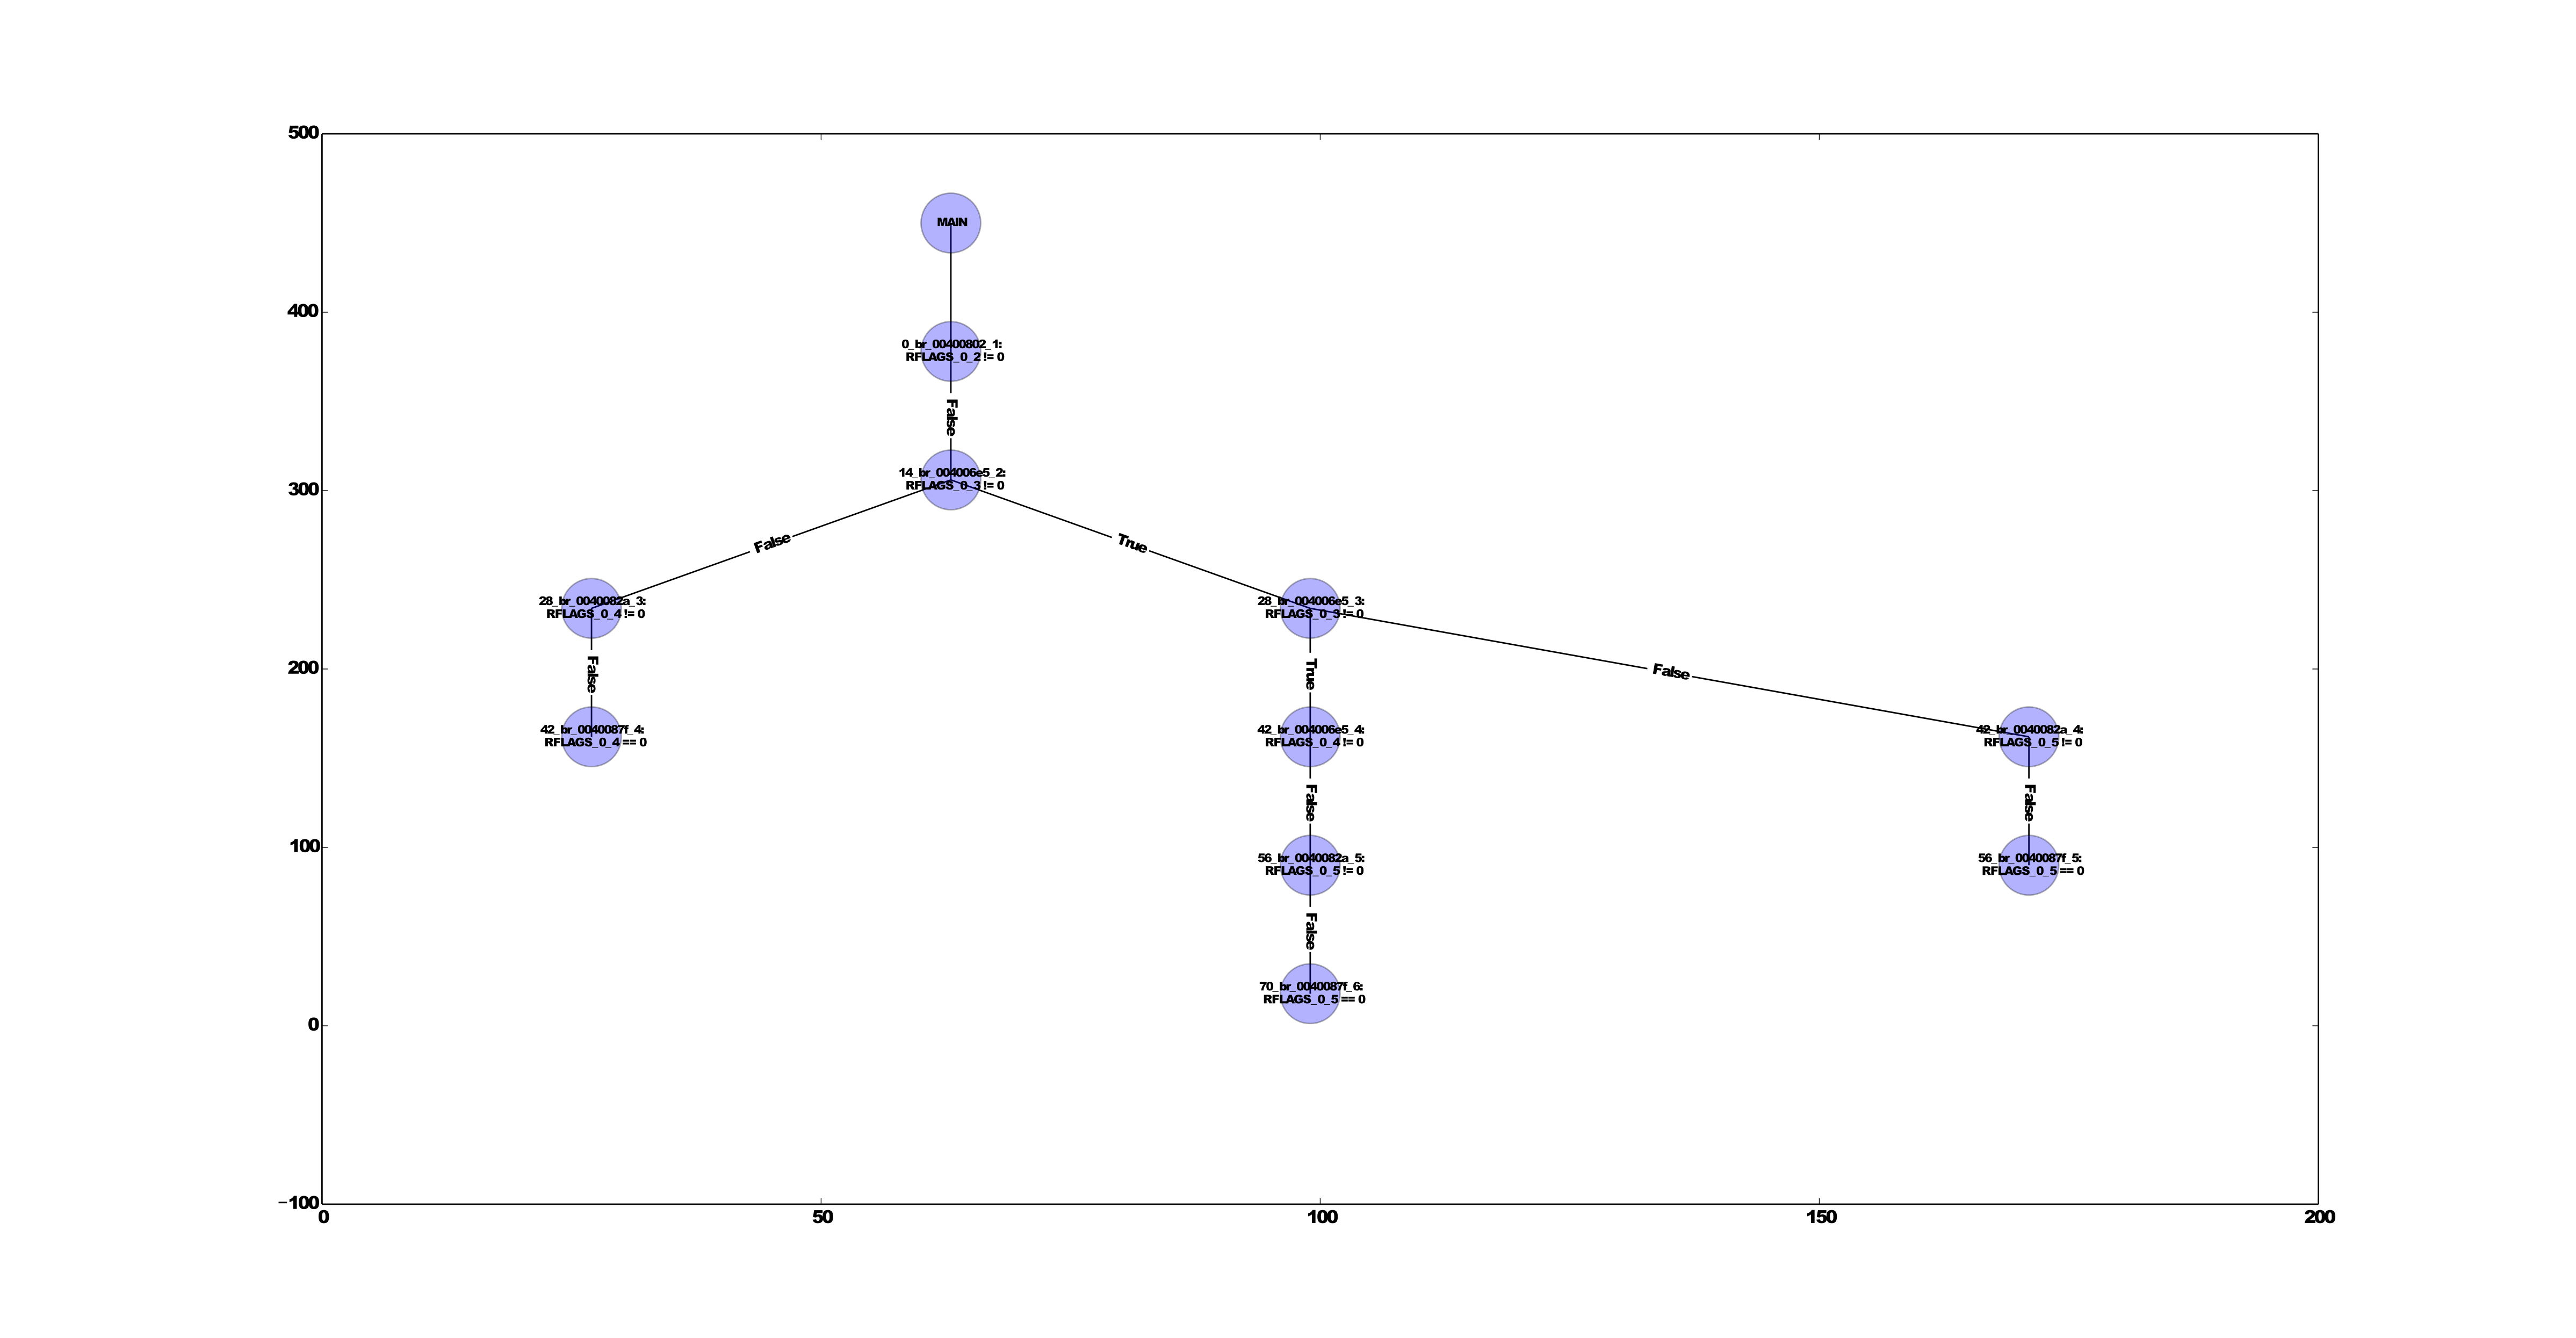
\includegraphics[width=0.45\textwidth]{graphs/1_5}\\\hline
   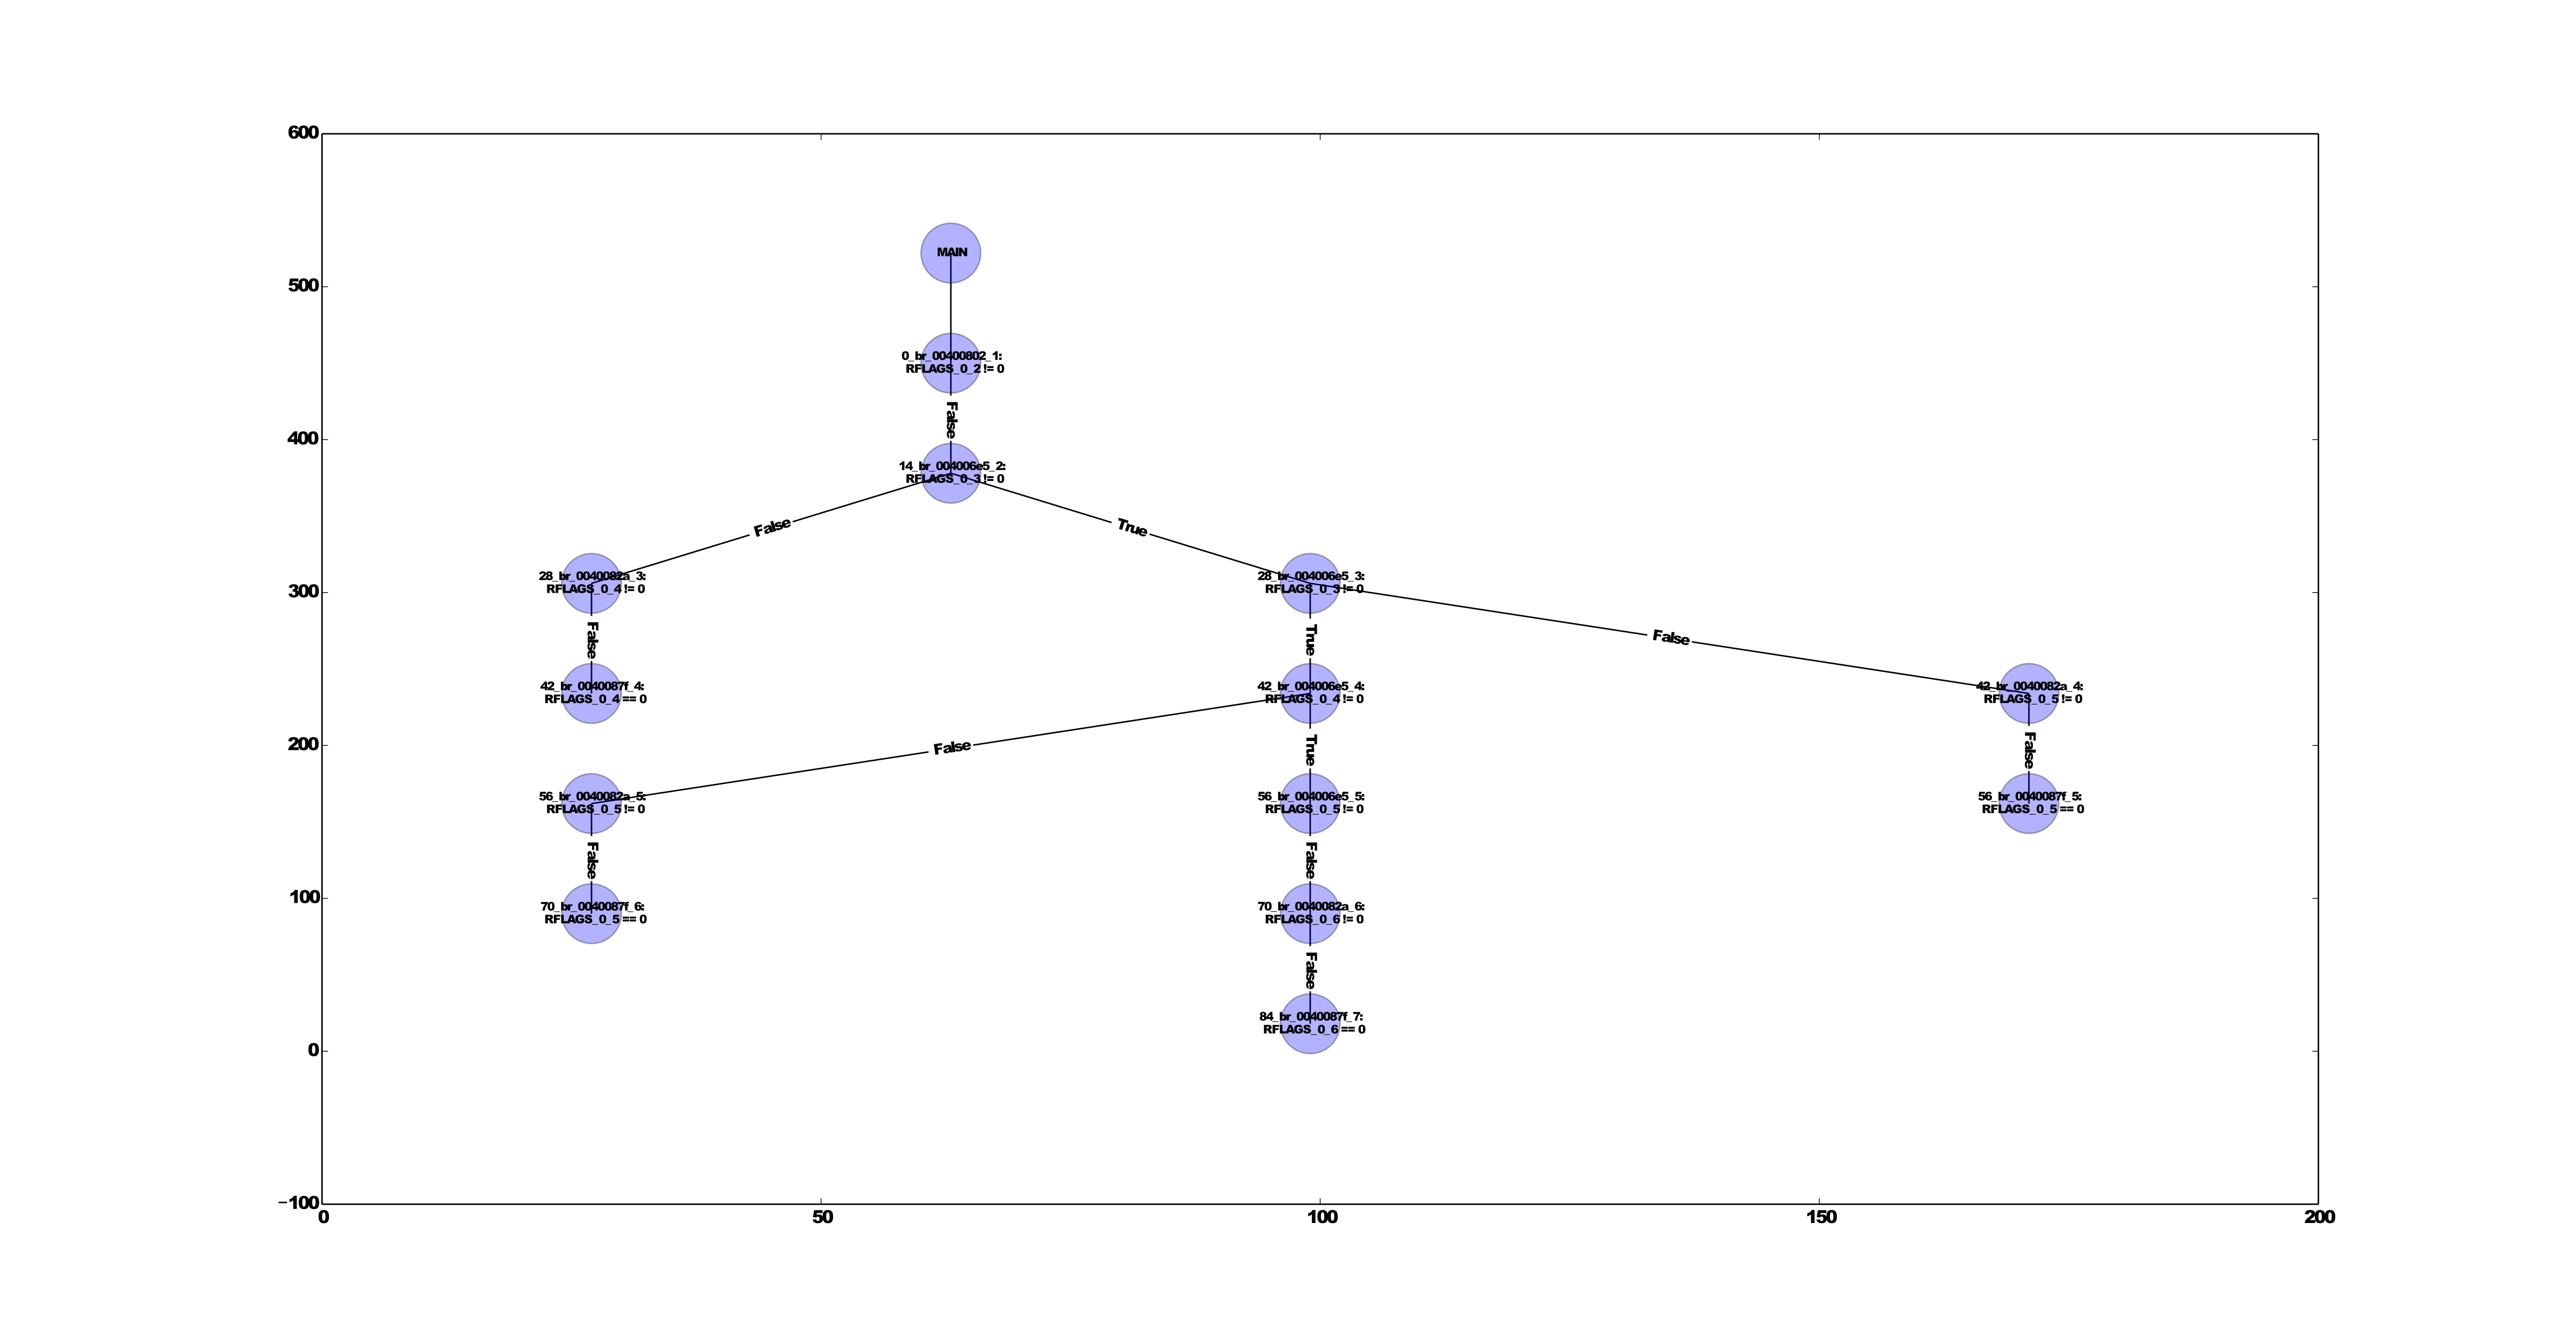
\includegraphics[width=0.45\textwidth]{graphs/1_6}
   &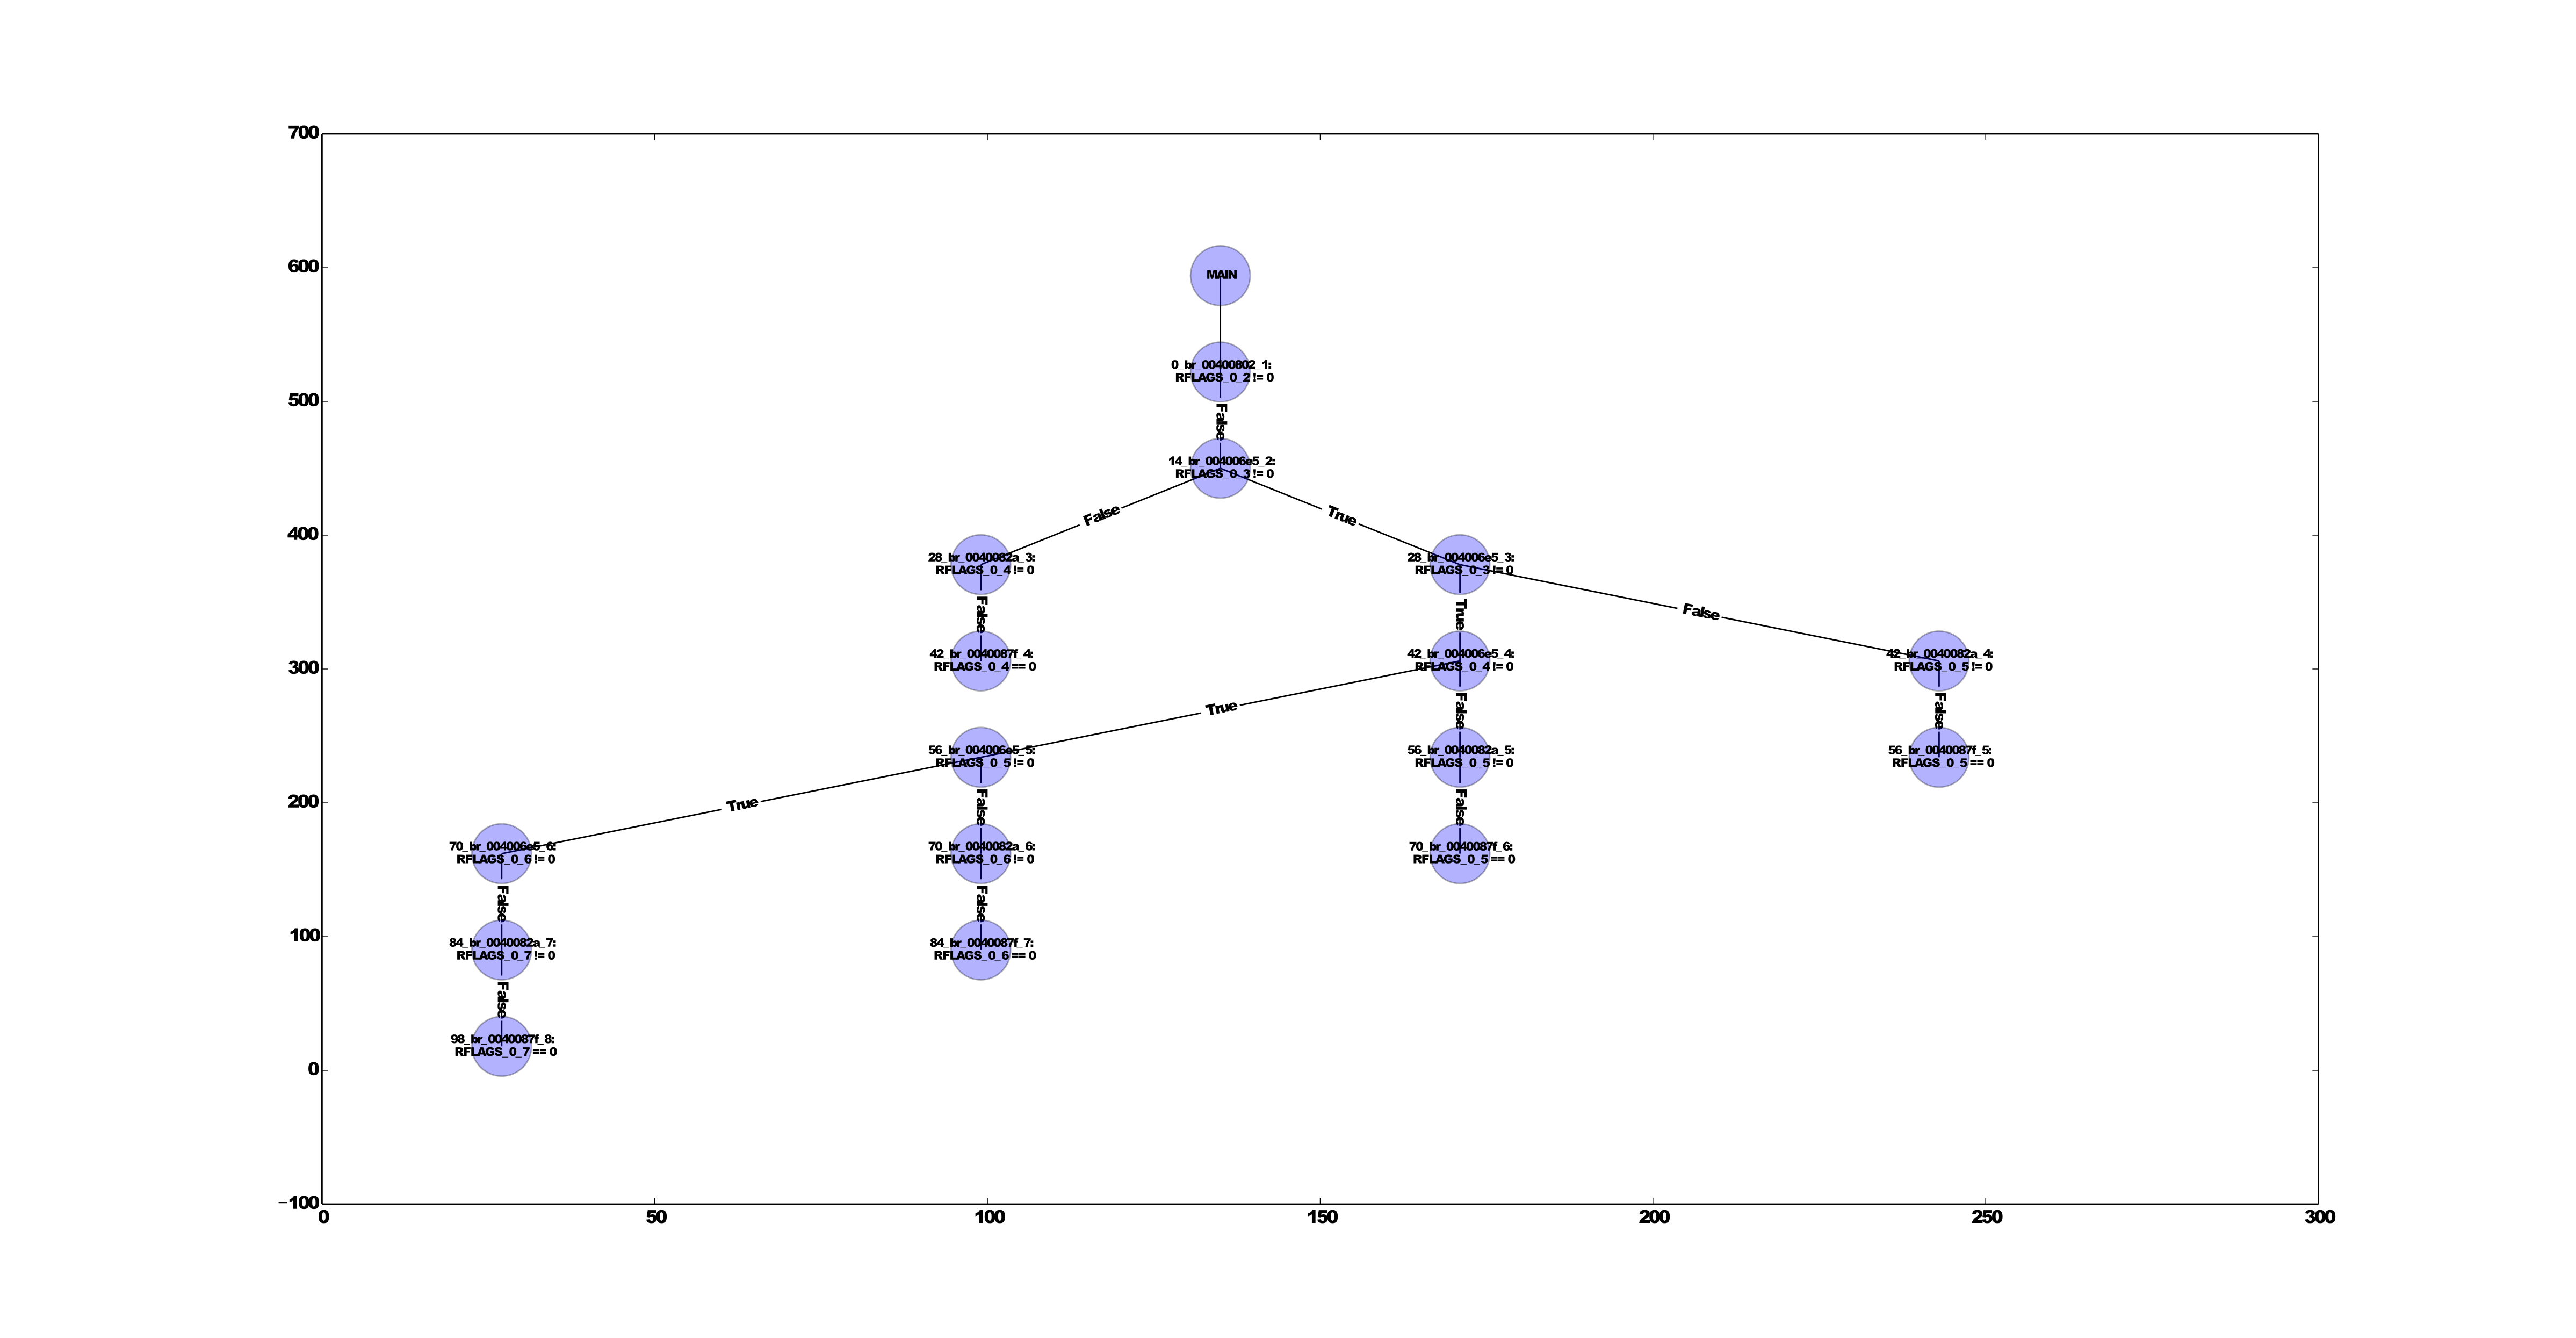
\includegraphics[width=0.45\textwidth]{graphs/1_7}\\\hline
 \end{tabular}
 \caption{Example Execution Graphs for test1}
 \label{figure:examplegraphs}
\end{figure}

\begin{figure}[ht]
 \centering
 \begin{tabular}{| c | c |}
   \hline
   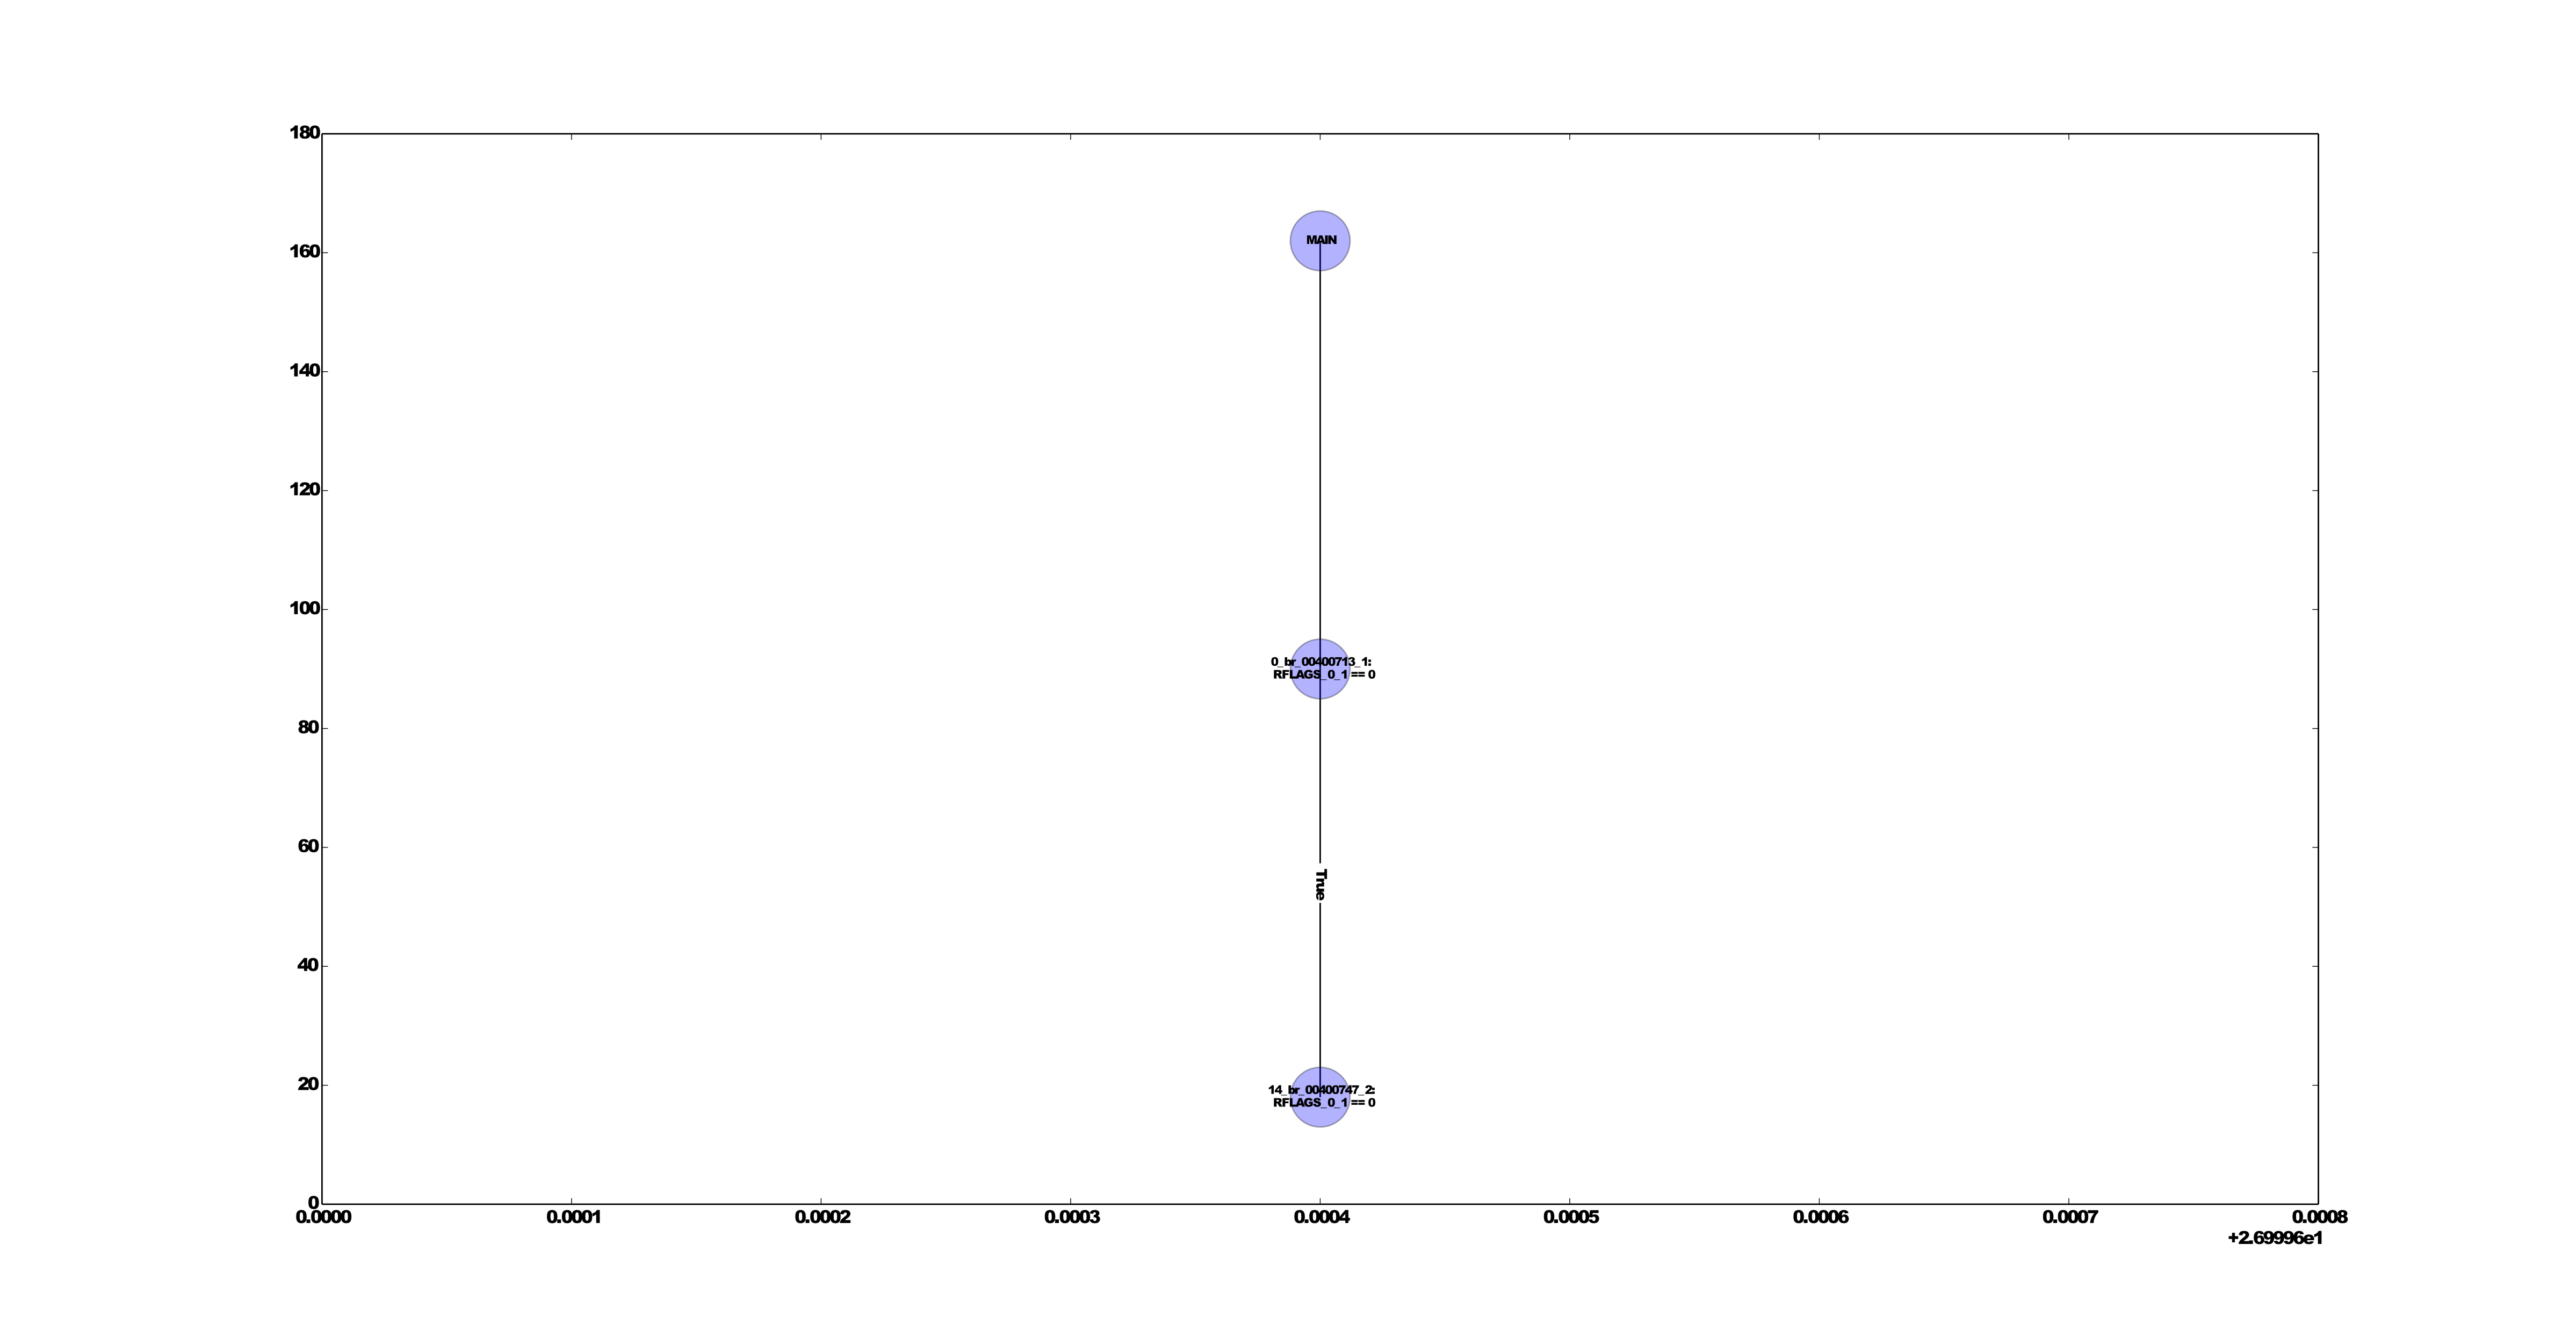
\includegraphics[width=0.45\textwidth]{graphs/2_0}
   &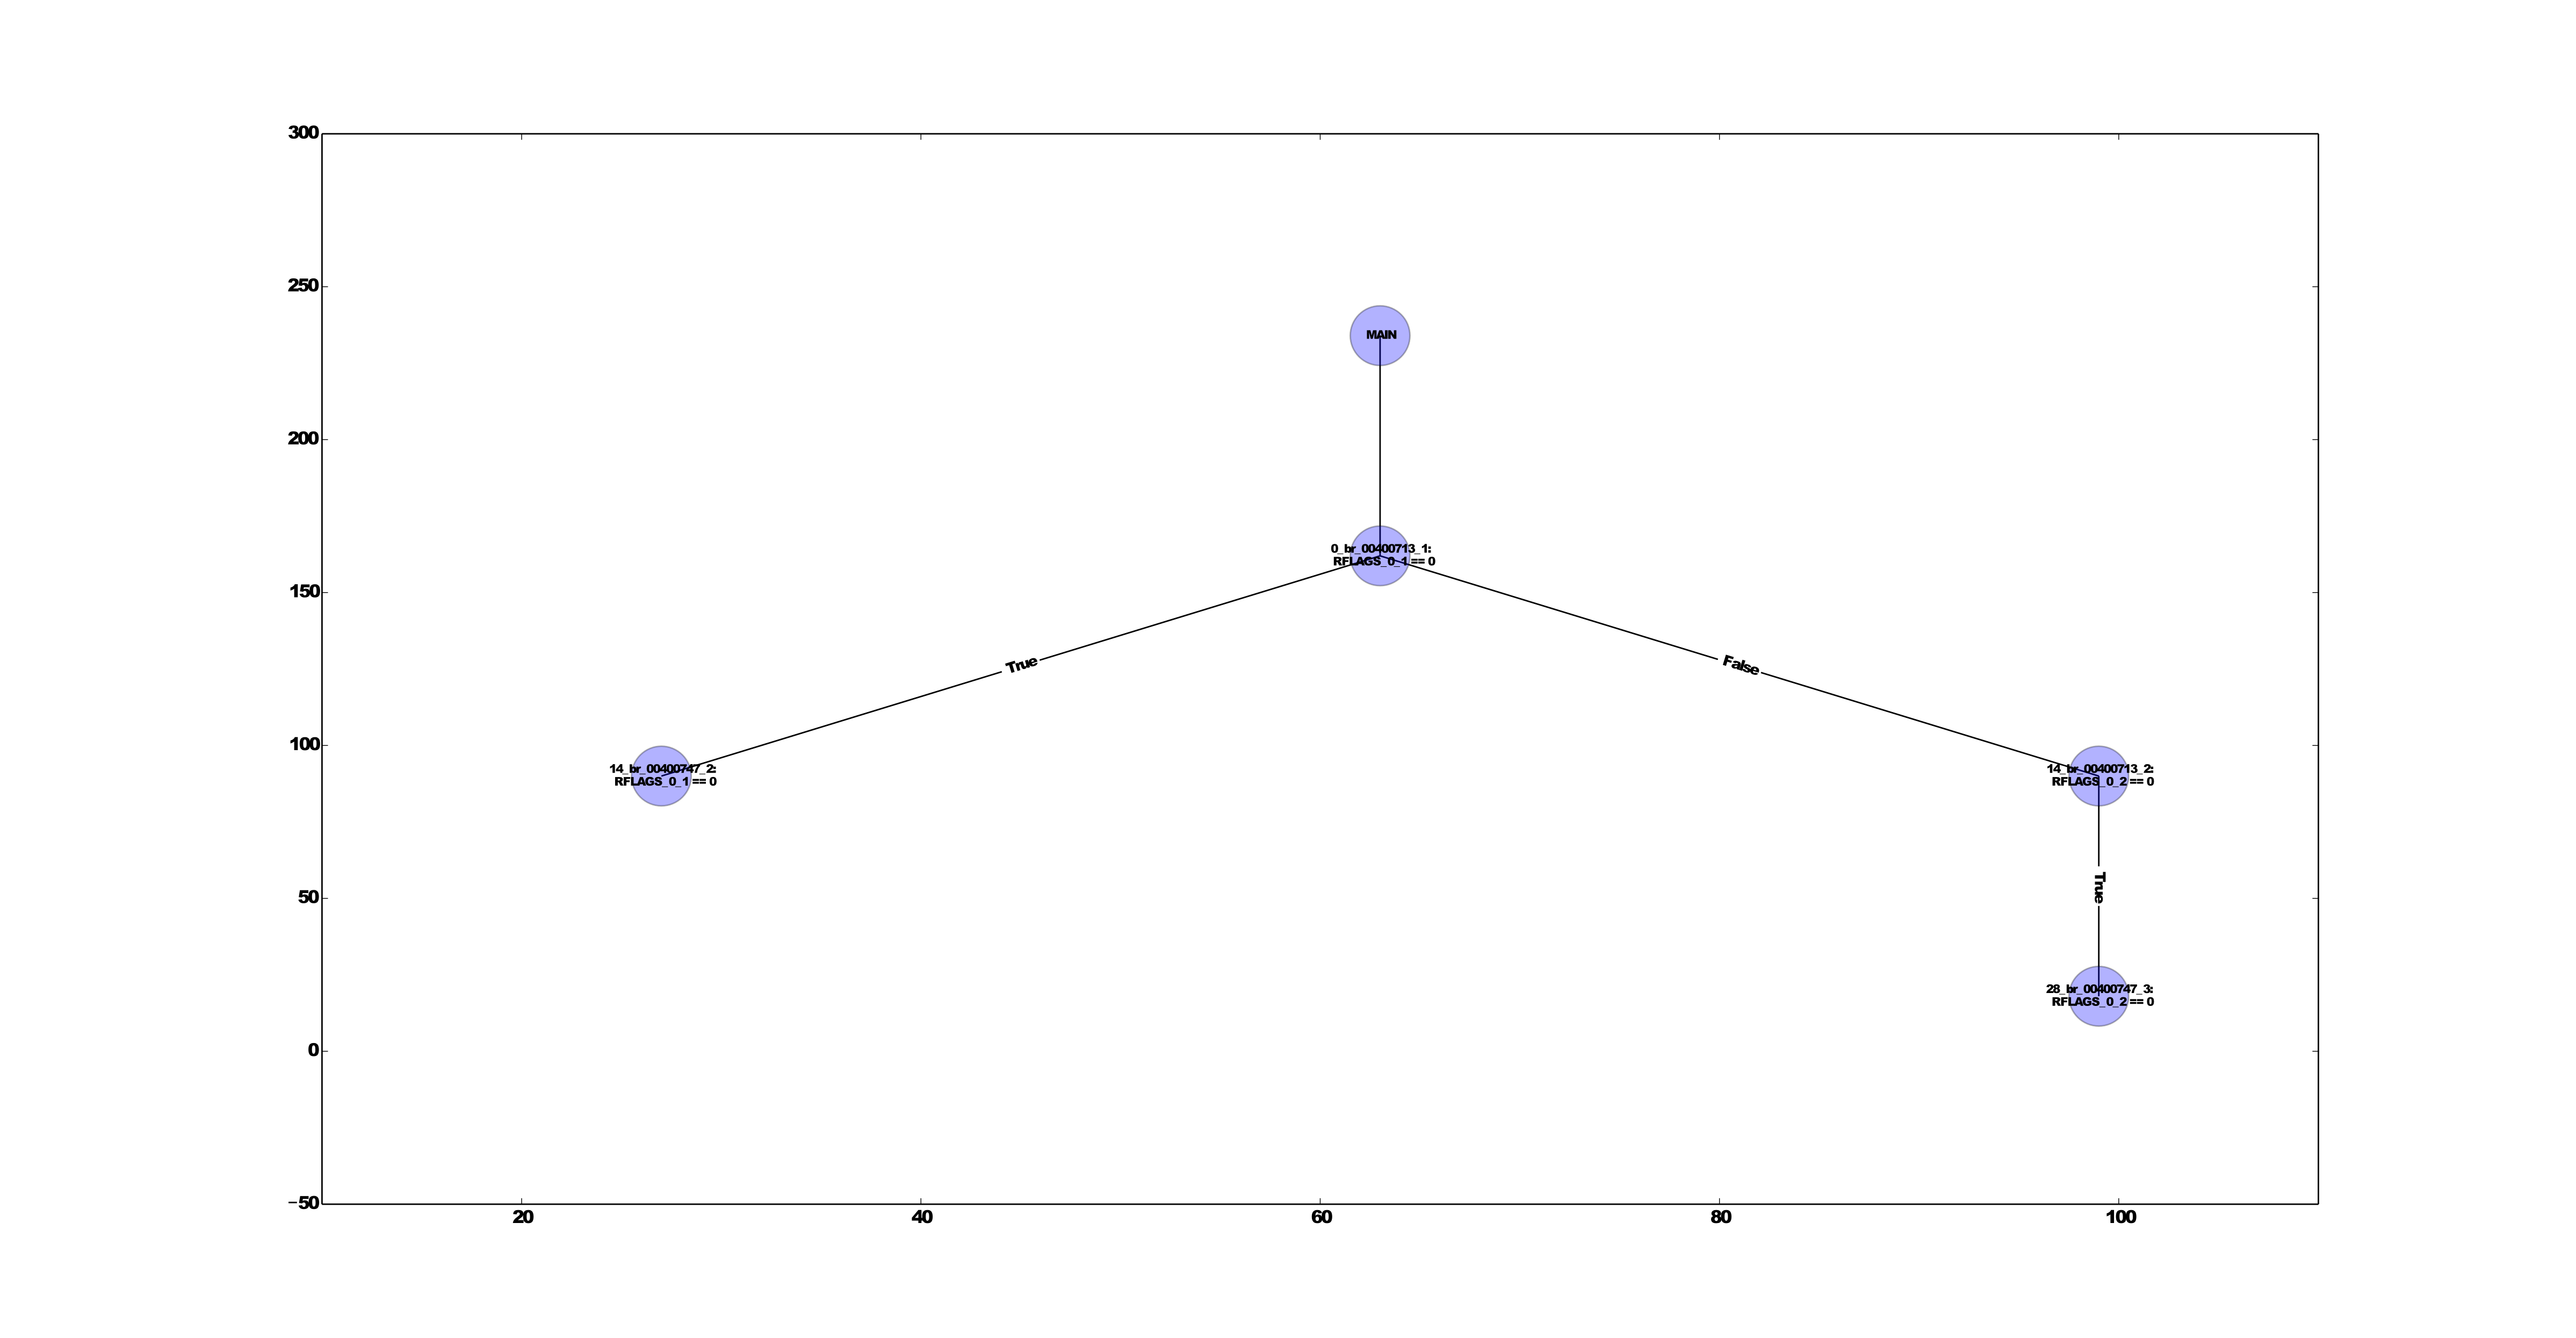
\includegraphics[width=0.45\textwidth]{graphs/2_1}\\\hline
   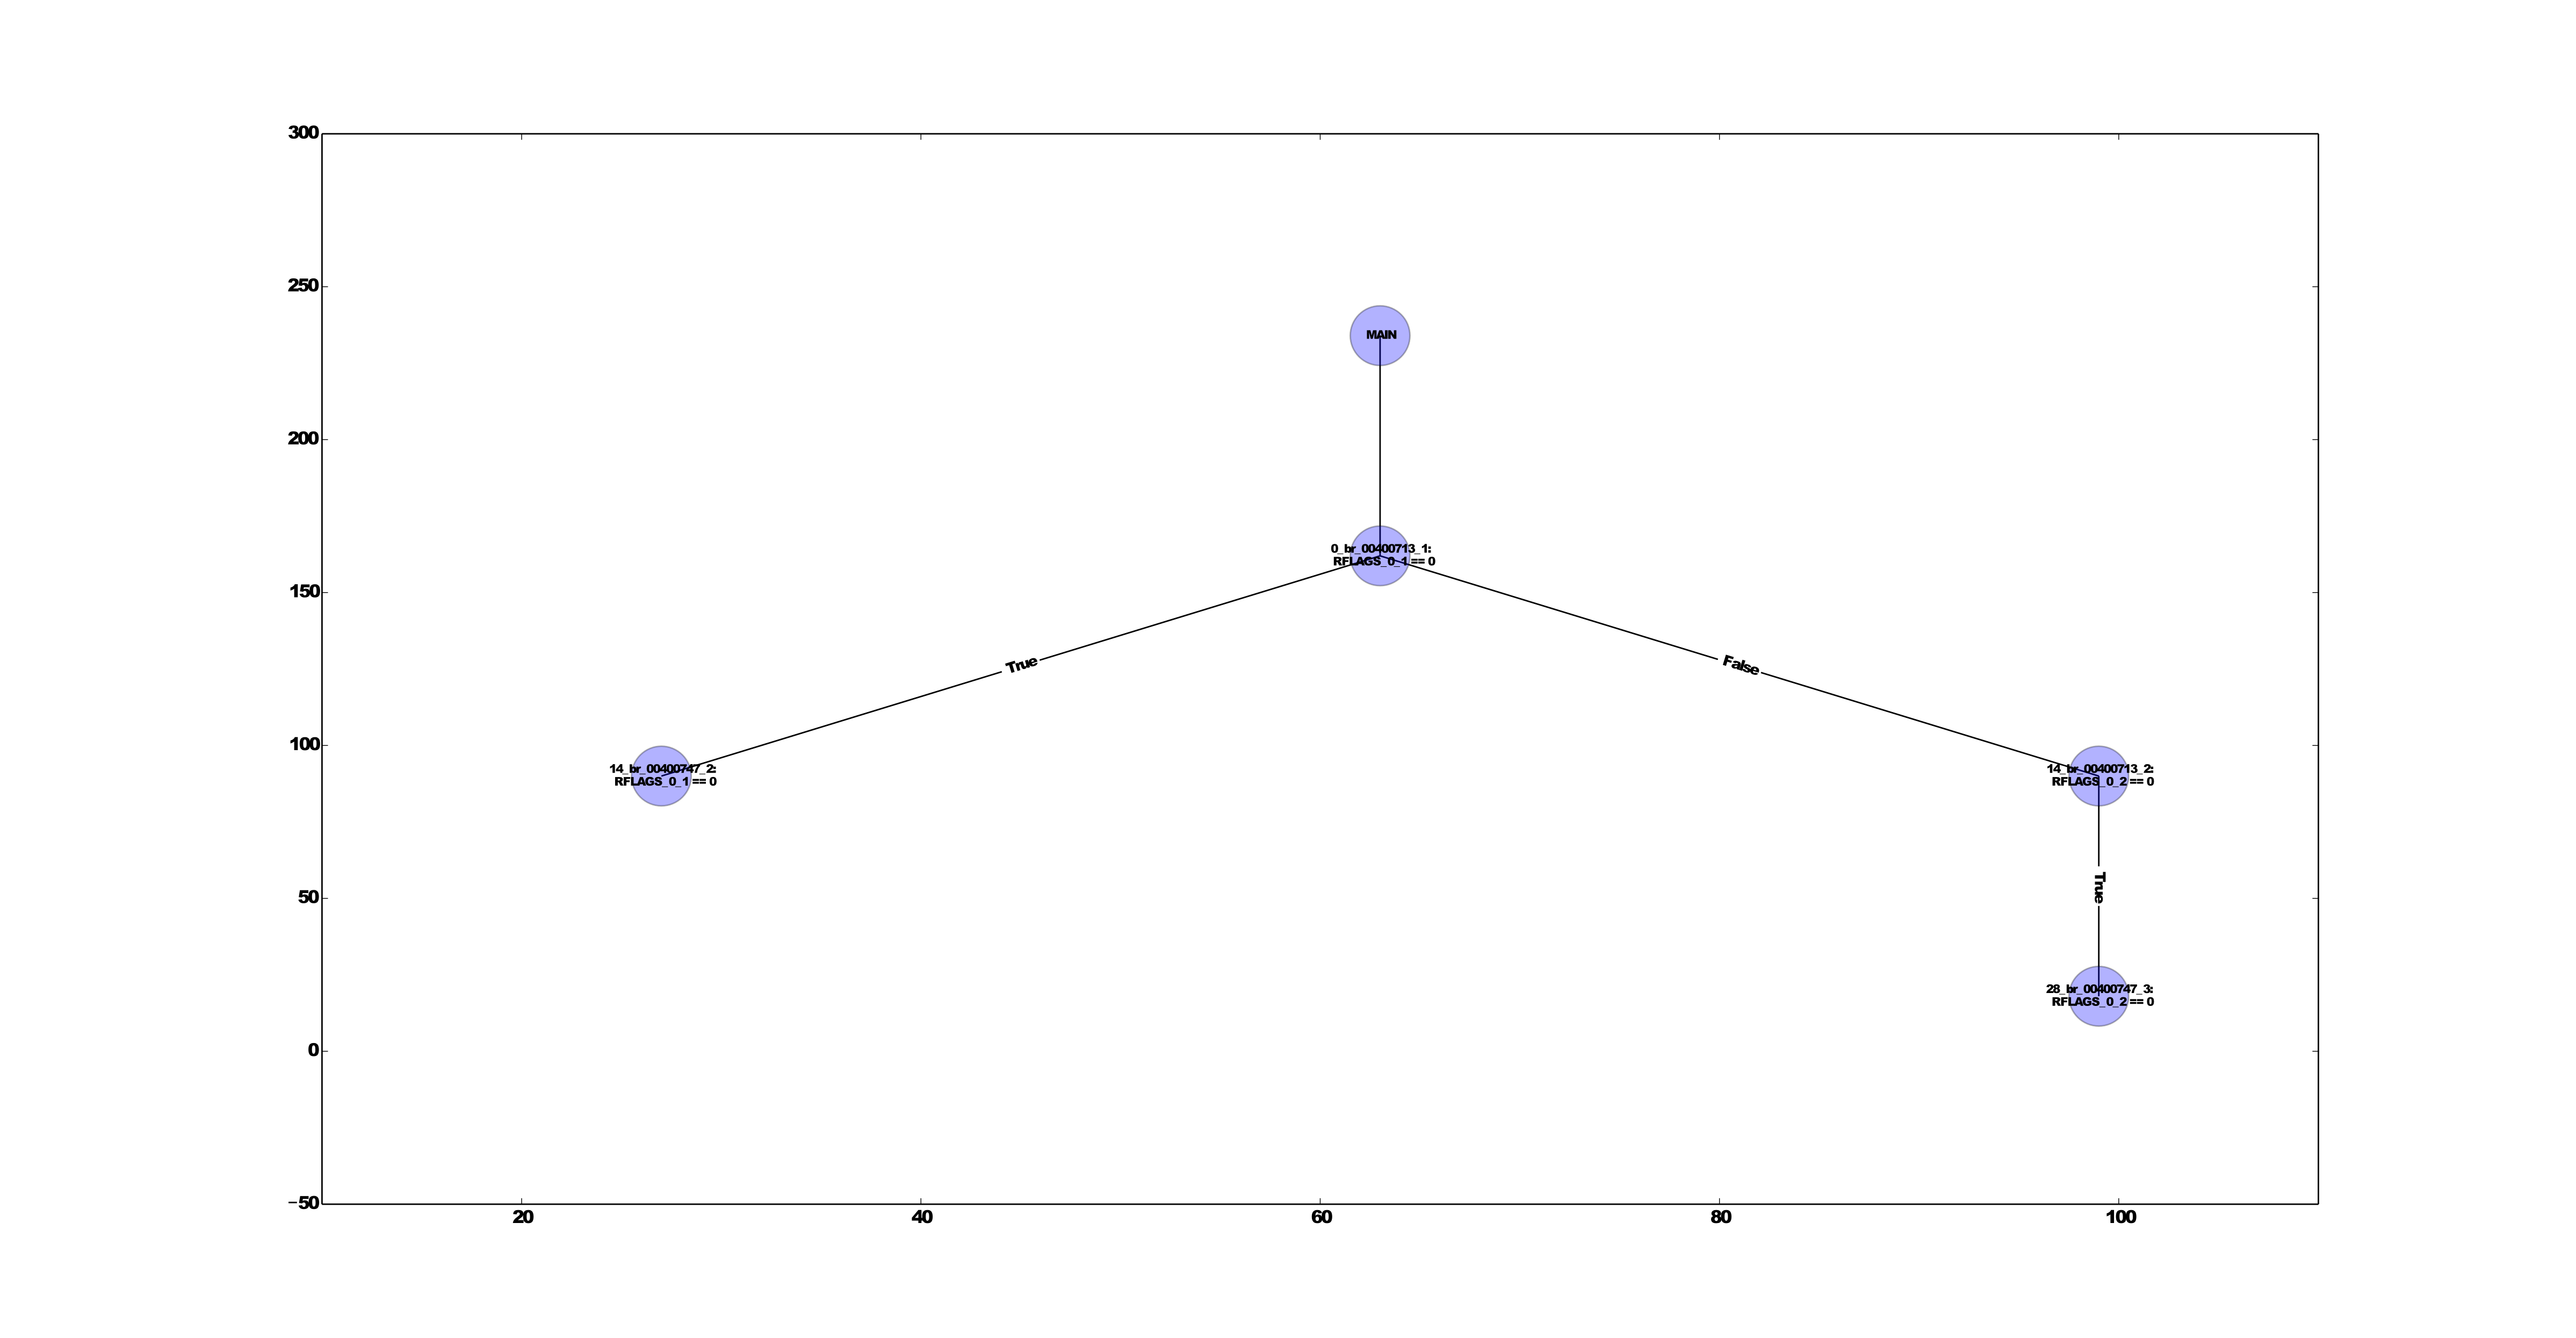
\includegraphics[width=0.45\textwidth]{graphs/2_2}
   &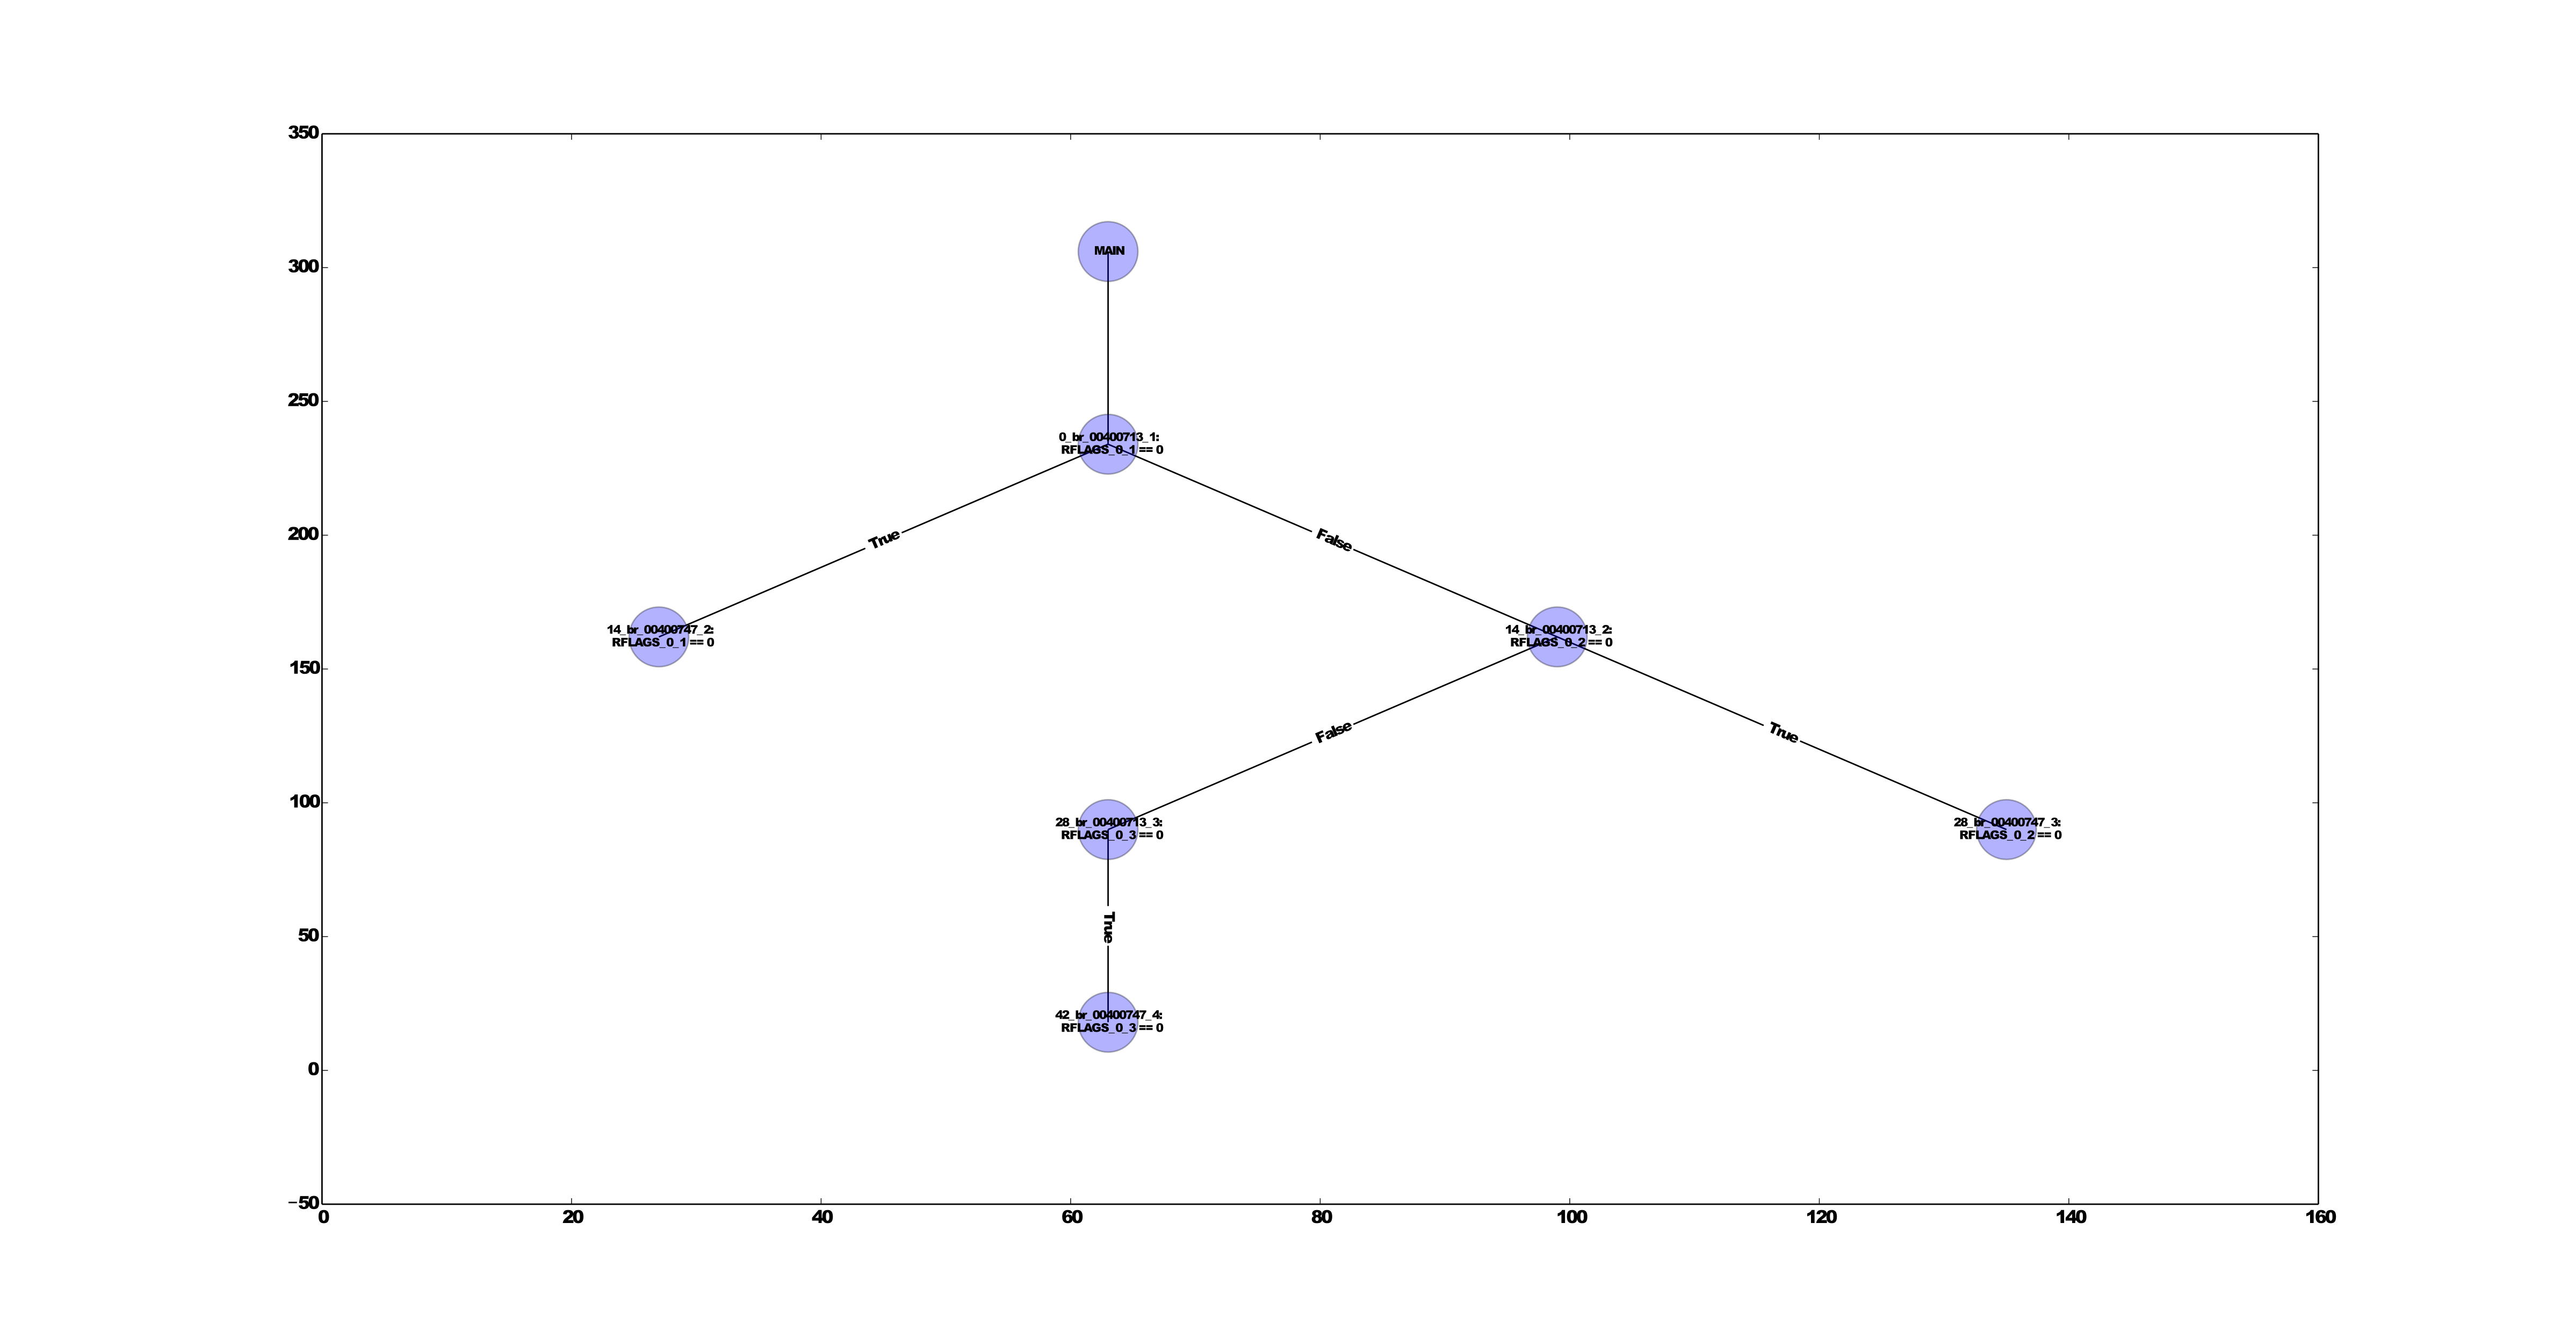
\includegraphics[width=0.45\textwidth]{graphs/2_3}\\\hline
   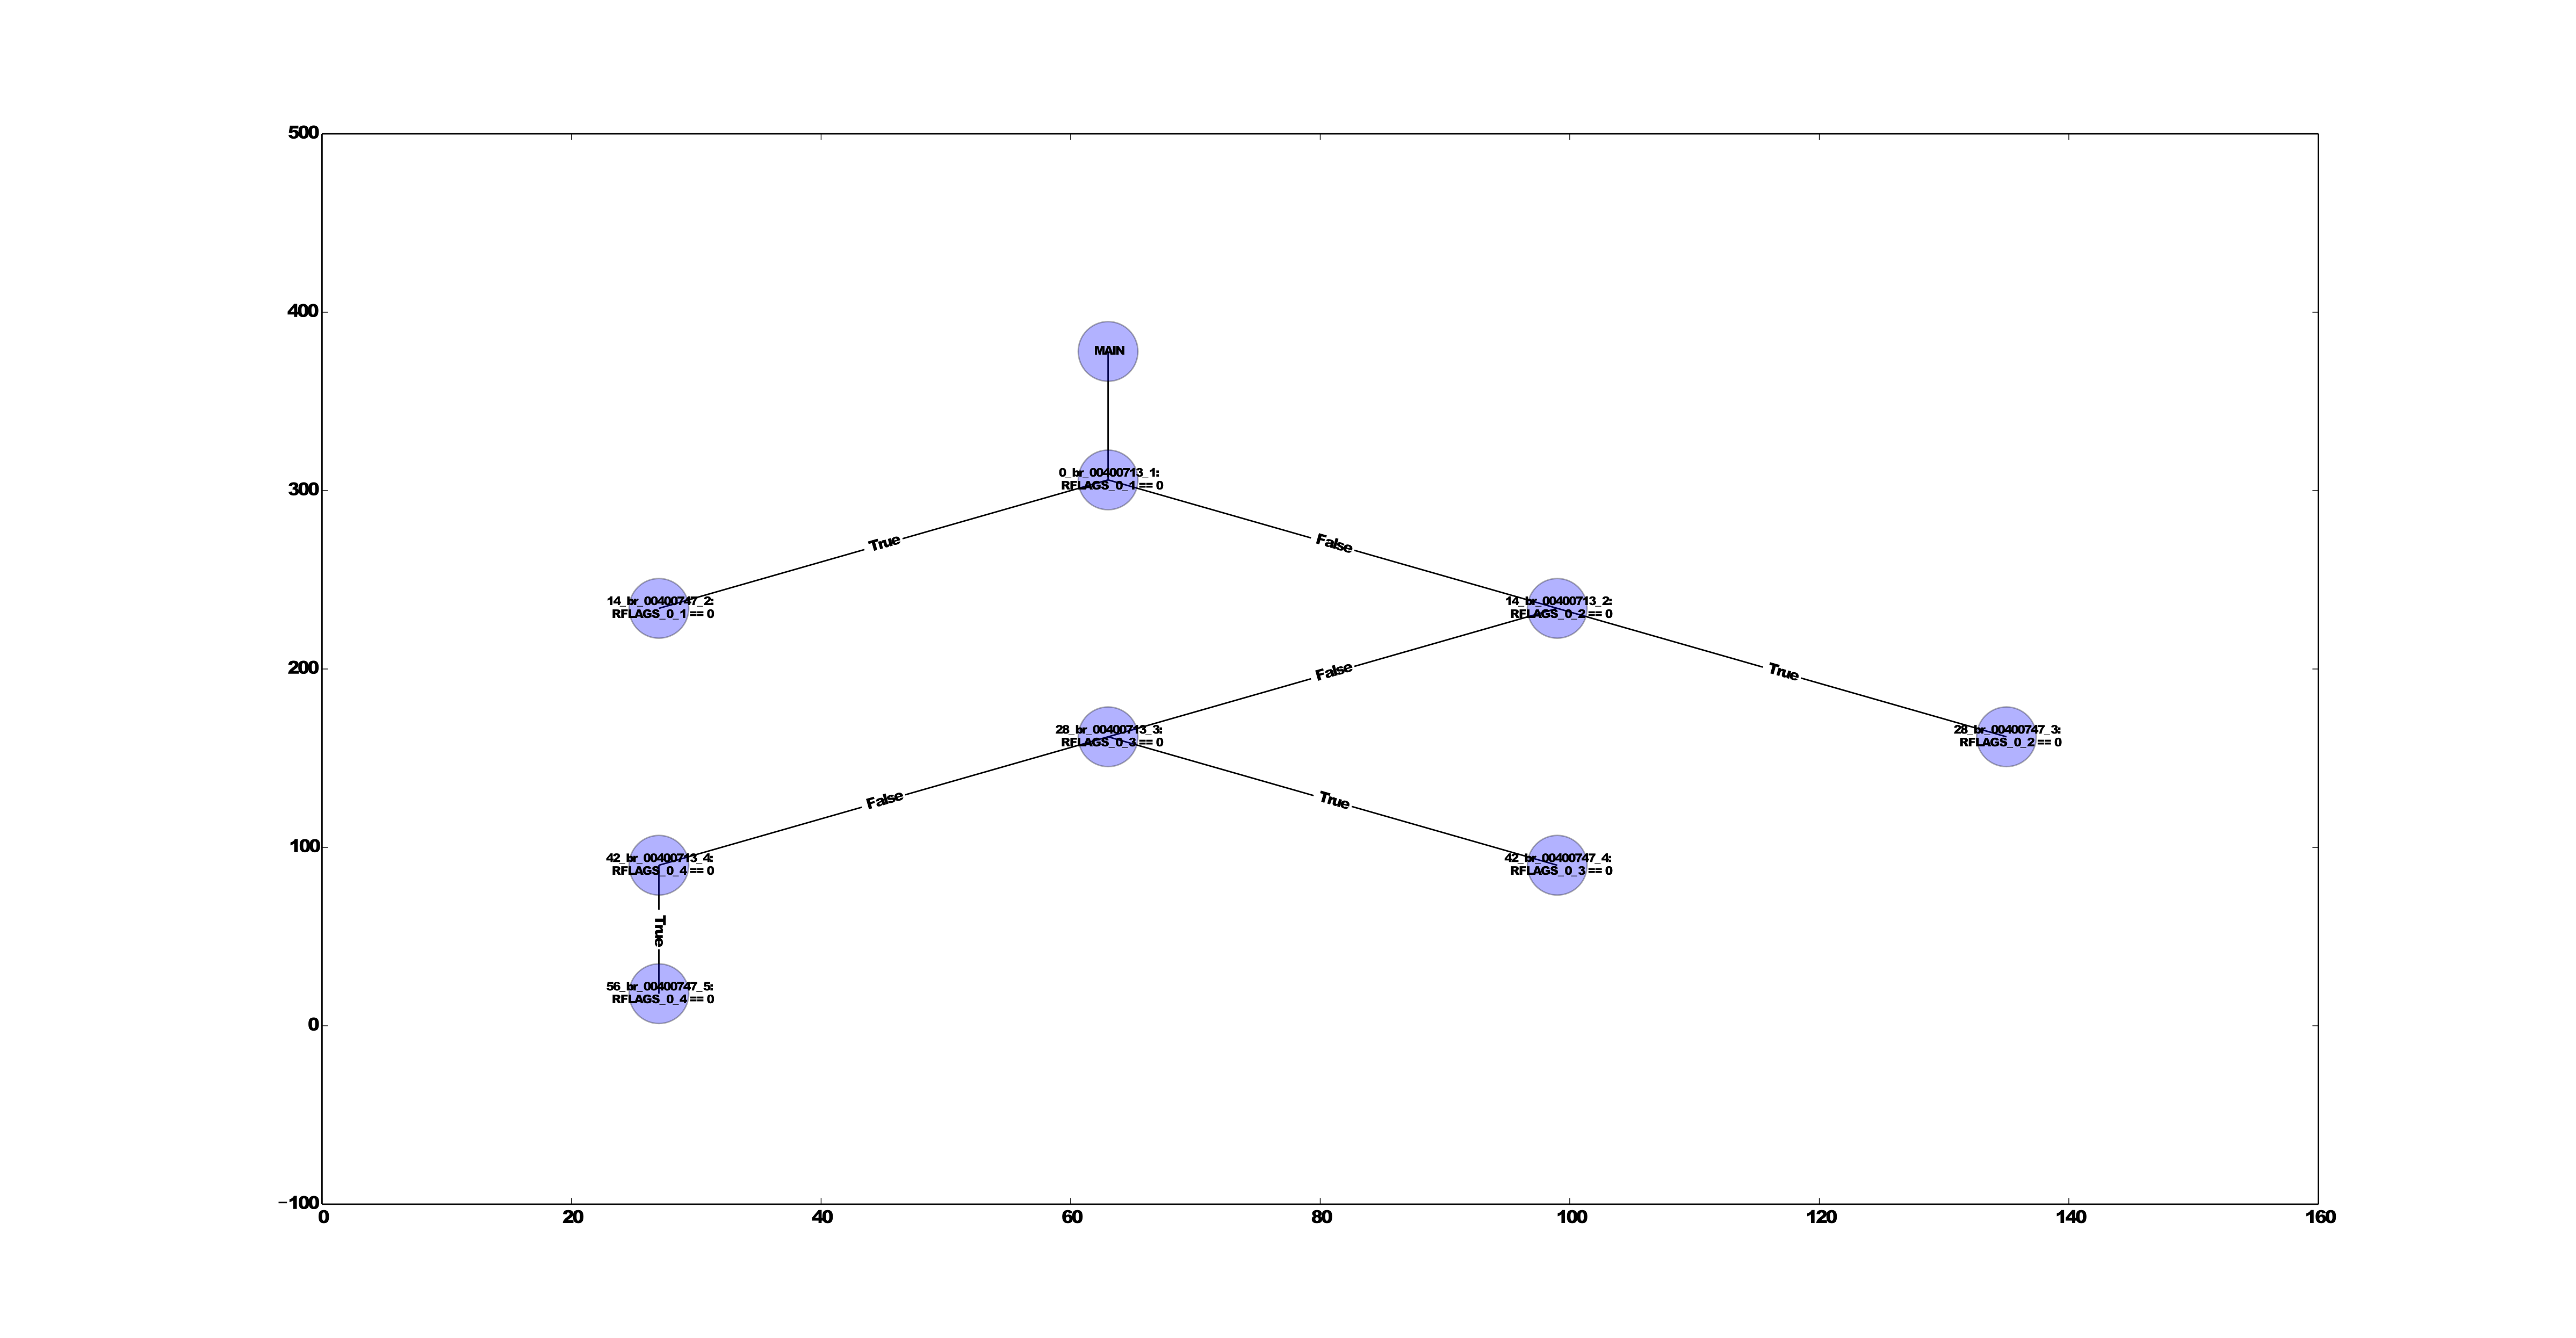
\includegraphics[width=0.45\textwidth]{graphs/2_4}
   &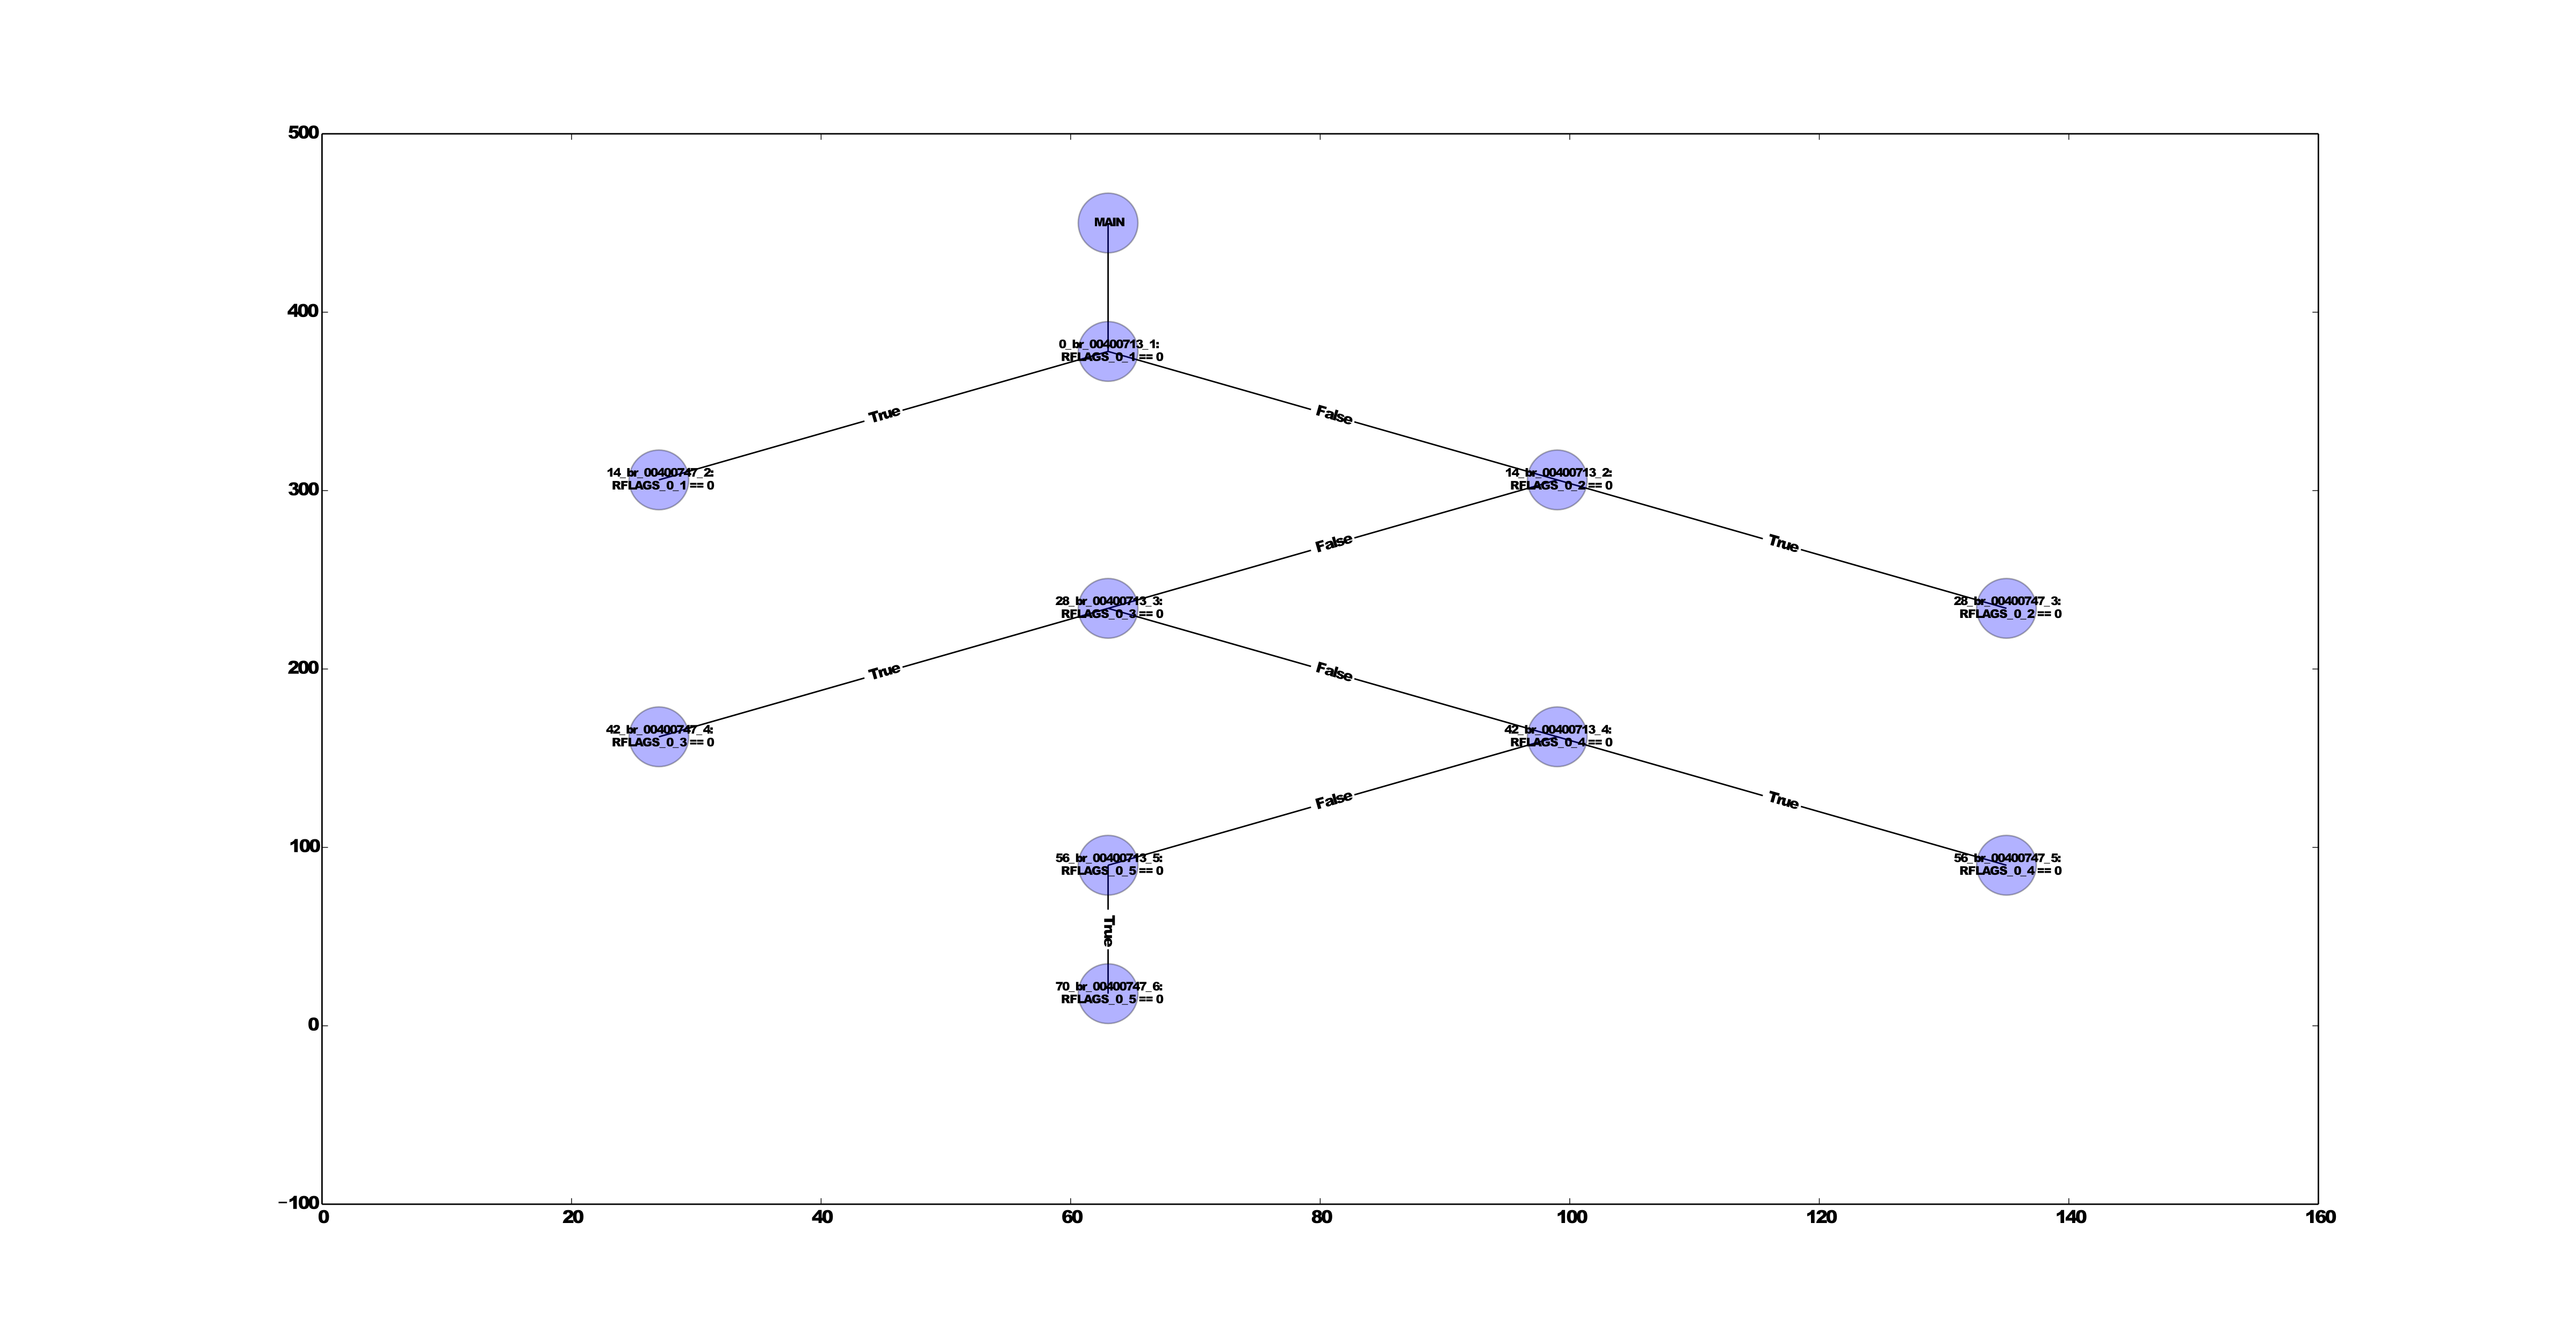
\includegraphics[width=0.45\textwidth]{graphs/2_5}\\\hline
   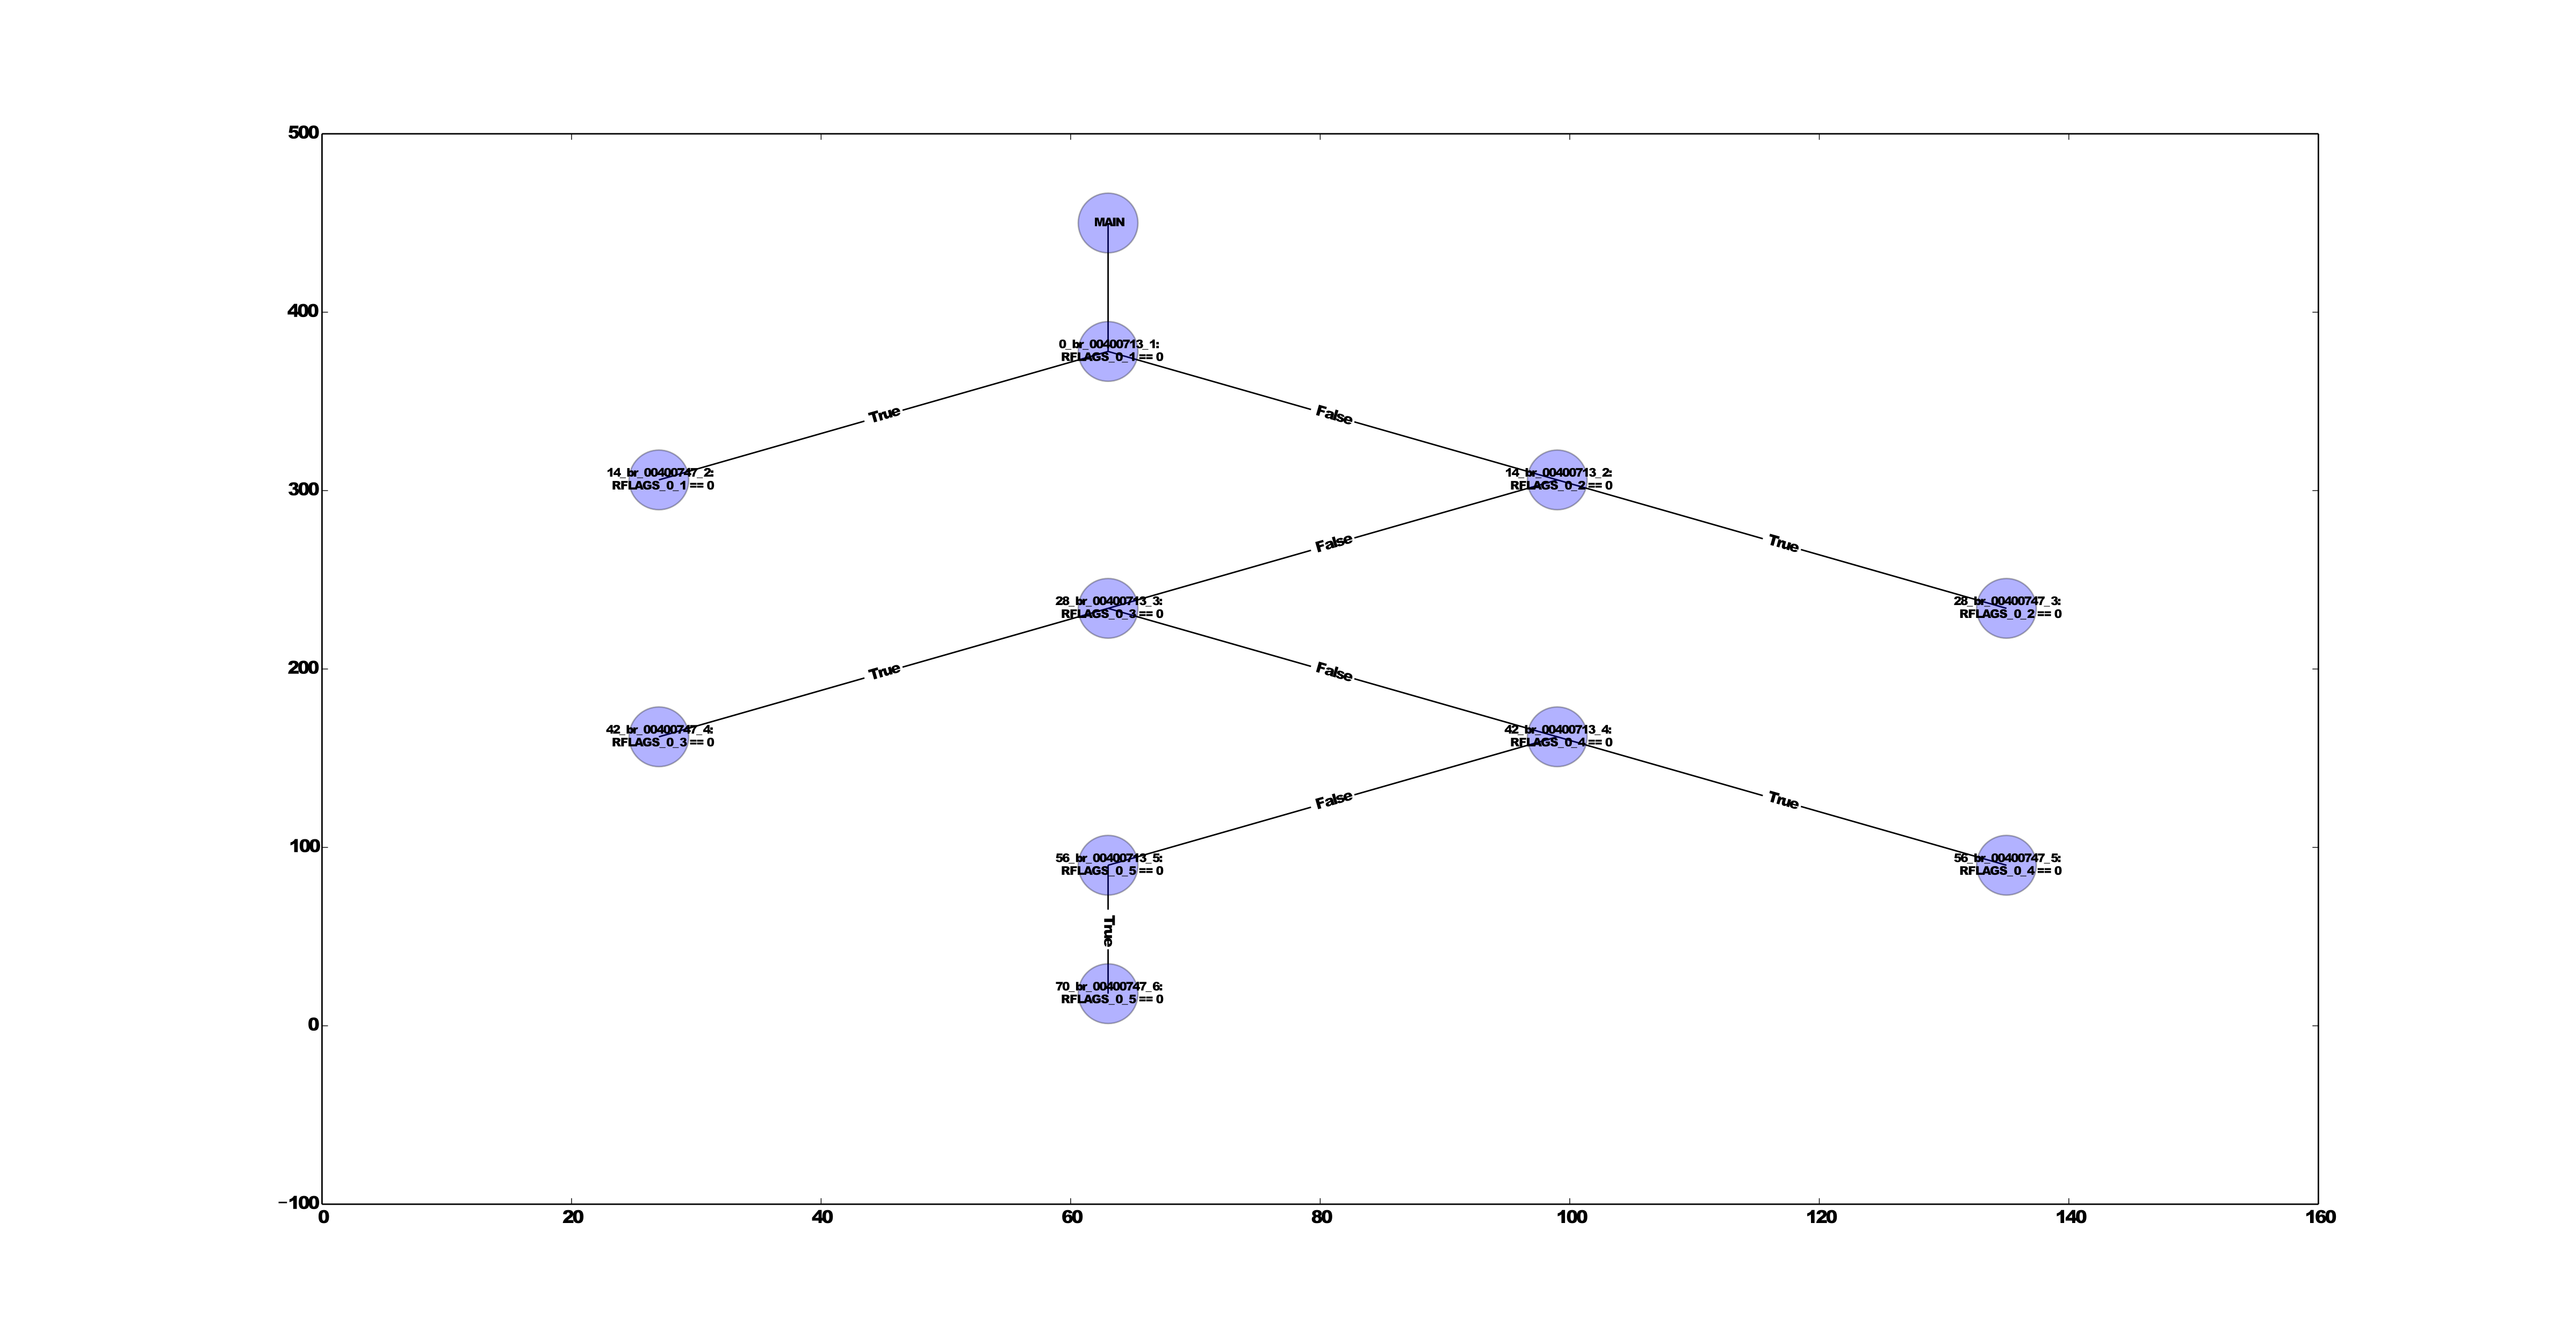
\includegraphics[width=0.45\textwidth]{graphs/2_6}
   &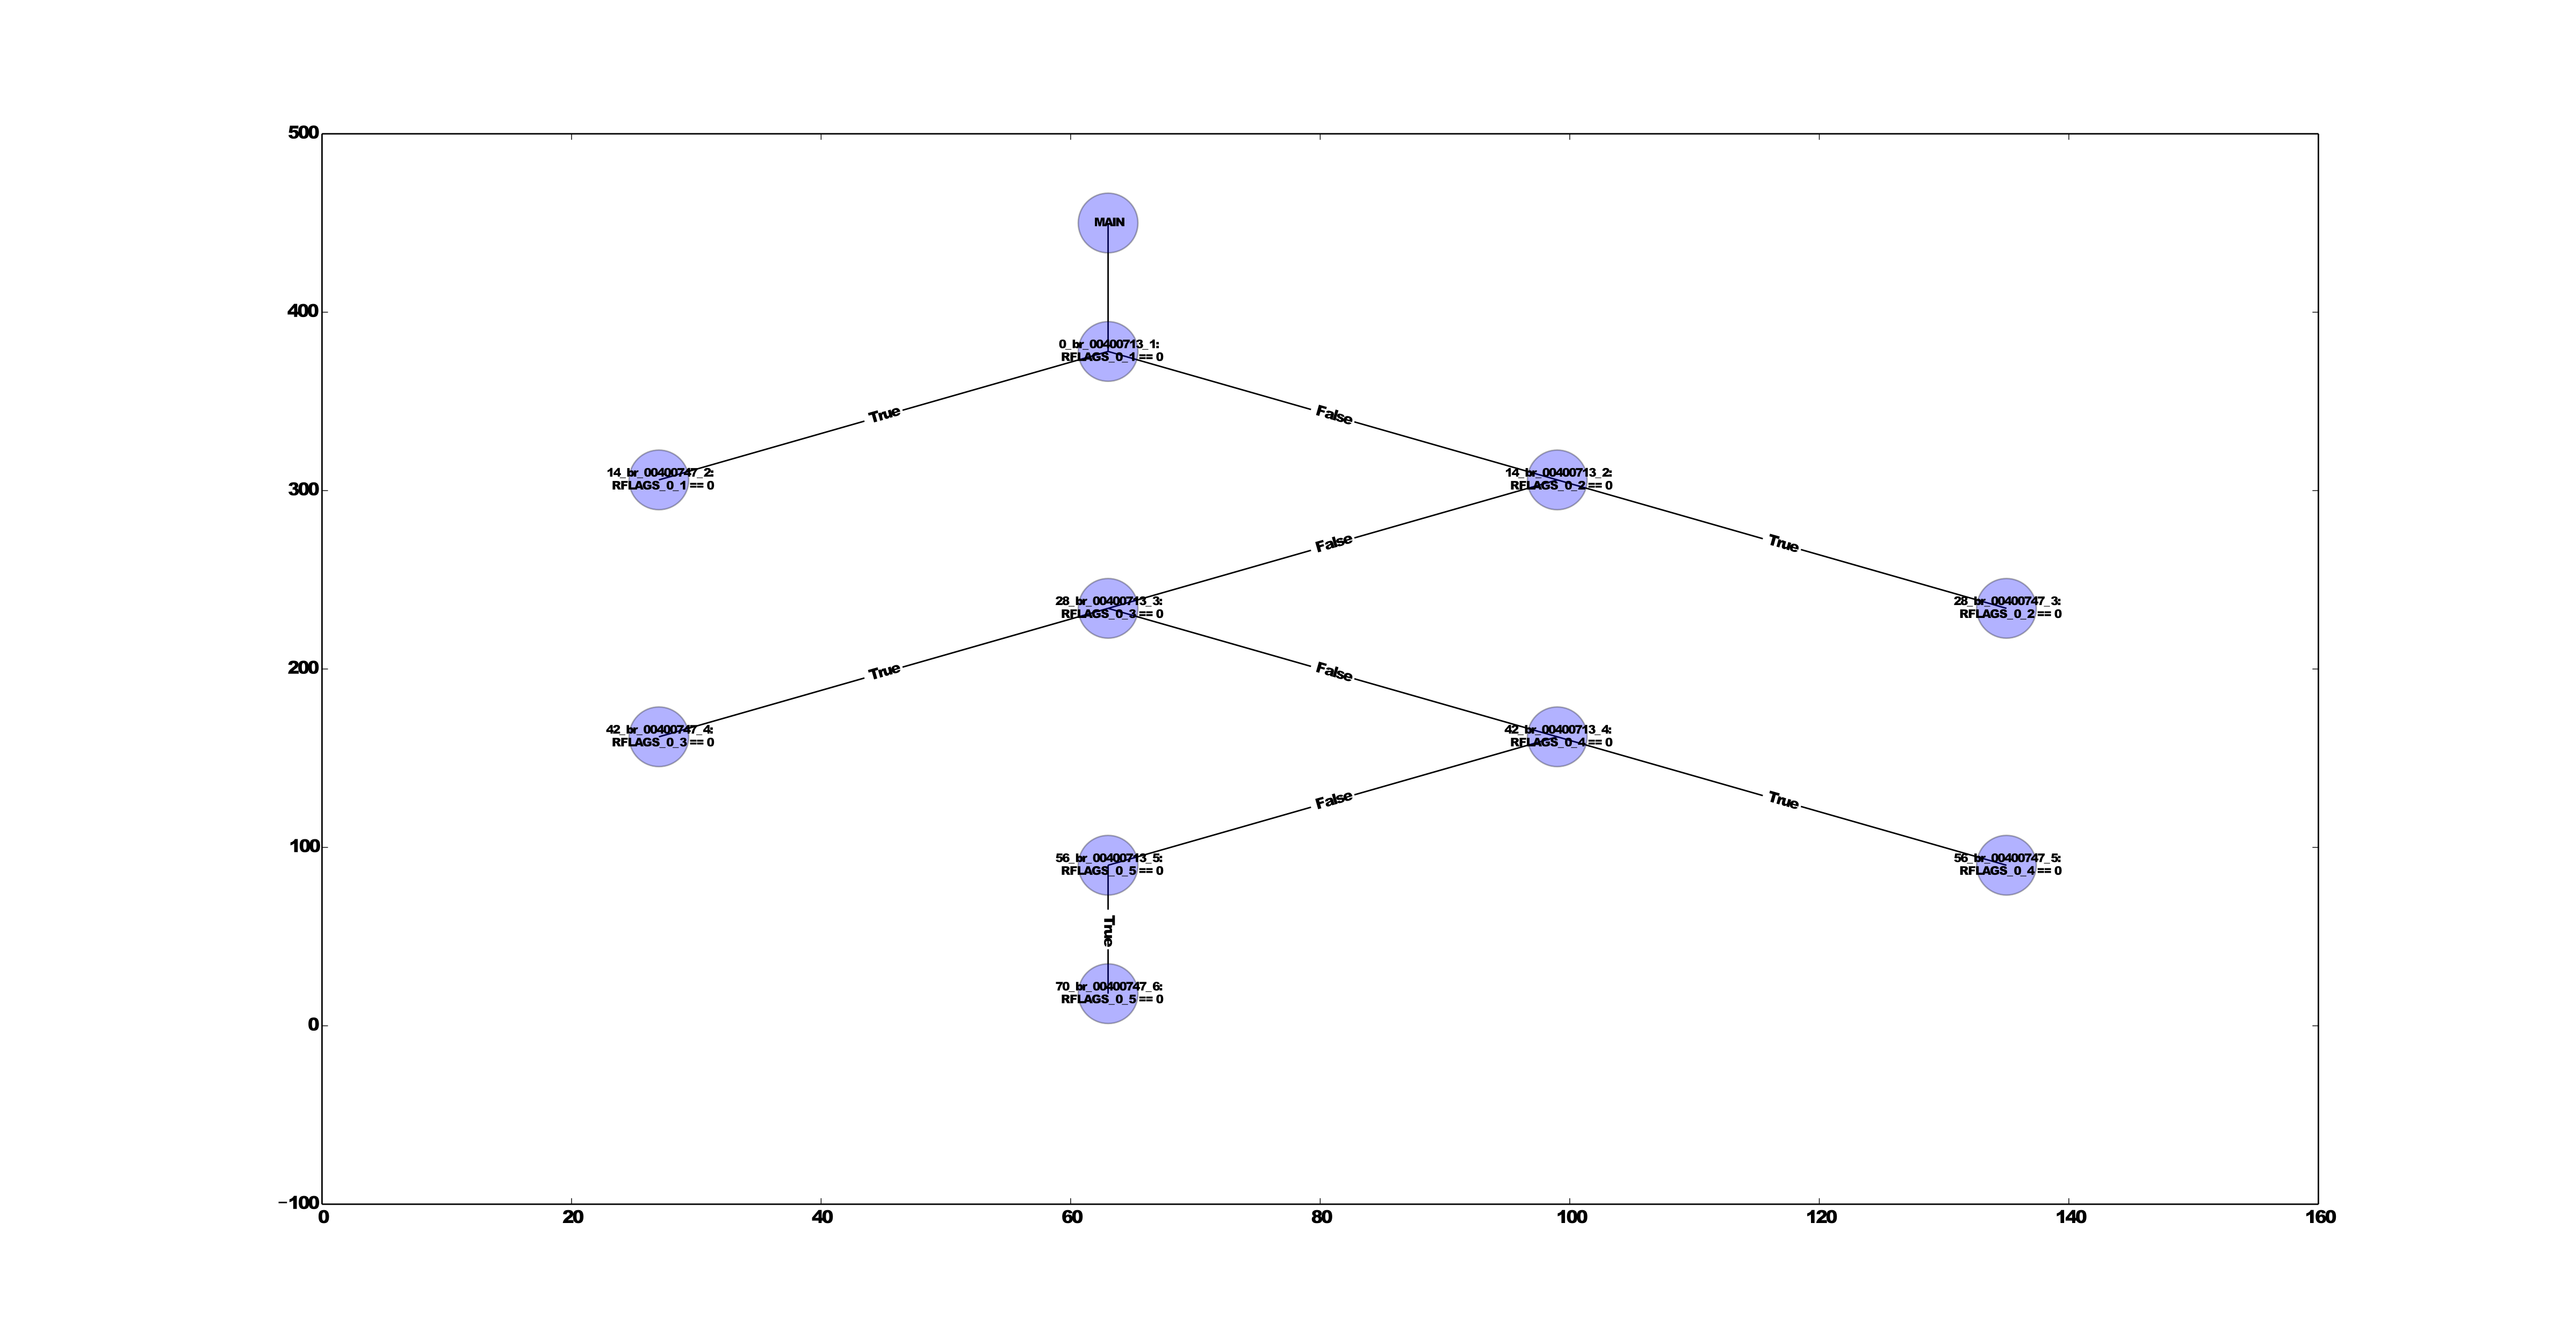
\includegraphics[width=0.45\textwidth]{graphs/2_7}\\\hline
 \end{tabular}
 \caption{Example Execution Graphs for test2}
 \label{figure:examplegraphs2}
\end{figure}

%% This defines the bibliography file (main.bib) and the bibliography style.
%% If you want to create a bibliography file by hand, change the contents of
%% this file to a `thebibliography' environment.  For more information 
%% see section 4.3 of the LaTeX manual.
\begin{singlespace}
\bibliography{main}
\bibliographystyle{plain}
\end{singlespace}

\end{document}

